%\documentclass{cumcmthesis}
\documentclass[withoutpreface,bwprint]{cumcmthesis} %去掉封面与编号页,电子版提交的时候使用。
\usepackage[superscript]{cite}
\usepackage{booktabs}
\usepackage{longtable}
\usepackage{float}
\usepackage{graphicx}
\usepackage{float}
\usepackage[framemethod=TikZ]{mdframed}
\usepackage{url}   % 网页链接
\usepackage{subcaption} % 子标题
\usepackage[linesnumbered,ruled,vlined]{algorithm2e} 
\usepackage{adjustbox}
\usepackage{algpseudocode}
\usepackage{longtable}


\title{电子产品的序贯抽检与多阶段策略优化}
 
\begin{document}
\maketitle
\begin{abstract}
	电子产品生产线面临零部件次品率、生产过程抽检及次品率、产品退换与拆解回收等多重质量控制问题。
	本文针对以上问题,构建了基于序贯概率比检验$SPRT$\cite{SPRT},
	优化算法和高斯过程的综合决策模型。该模型通过动态调整零部件抽样方案、优化生产过程中的检测与拆解策略,
	并在考虑次品率波动的情况下,最大化生产净利润。实验结果验证了模型在降低抽检成本、提高决策效率和增强鲁棒性方面的有效性。

	针对问题一提出的零部件抽样验收问题,本文构建了基于序贯概率比检验\textbf{$SPRT$}的动态抽样决策模型,
	利用给定的标称次品率与引入的扰动量构建零假设与备择假设下的似然函数以拟合问题设置的两种情况,
	进而确定\textbf{$SPRT$}的决策边界。为提升模型泛化能力,本文采用\textbf{多层感知机$MLP$}对扰动量进行函数拟合,最终实现在3\%以下抽样占比下对零部件批次做出平均
	精度超过90\%的决策。

	针对问题二,我们构建了包含零配件1、零配件2、成品是否检测以及成品是否拆解,共四个生产流程决策变量。对于题目中给出的6种情况,本文首先计算出了在不同情况下,投入零件在自然组合状态下组装得到次品数量的概率分布,确保每个生产周期投入生产的零件都符合对应的概率分布。本文模拟了在连续生产过程中所有可能的决策变量组合,以最大化单件成品的纯利润为目标,计算出了在每种情况下的最优决策方案以及对应的单件成品的纯利润。
	
	针对问题三,本文扩展了生产流程决策变量,包含了8个零件、3个半成品和1个成品的相关决策,共16个生产流程决策变量。本文首先计算出了投入零件在自然组合状态下组装得到不同半成品次品数量的概率分布,确保每个生产周期投入生产的零件都分别符合对应的概率分布。本文模拟了企业的连续生产过程,基于遗传算法,以最大化单件成品的纯利润为目标,计算出了最优决策方案以及对应的单件成品的纯利润。
	
	针对问题四,我们将各阶段由于抽样误差所引起的归纳误差建模为\textbf{马尔可夫过程},将单次的偏差量化高斯分布。通过\textbf{前向扩散}过程论证了误差传递策略
	的有效性。对于单次误差分布的建模,我们依据\textbf{$SPRT$}在多次二分采样后的误差与真实值的偏差作为样本值,通过对样本序列的最大似然估计回归出
	单次误差分布,通过对问题二和三的优化模型引入该误差分布,我们获得了更具备鲁棒性的决策方案。

	\noindent{ \textbf{关键词:} $SPRT$\quad  多层感知机\quad 遗传算法\quad 马尔可夫过程\quad 前向扩散过程}
\end{abstract}


\section{问题重述}
某电子产品的生产企业需要综合诸多考虑购置零部件、产品抽检、产品拆解、报废等问题,以确保产品质量的同时降低成本。

\textbf{问题一:}考虑到零配件供应商所述次品率不高于既定标称值,企业拟采用抽样检测方法以验收此批零配件。因为企业寻承担检测费用,企业希望应用数学模型得到最少抽检次数的抽样方案。

已知标称值为 10\%,结合以下两种不同情况,分别设计出具体的抽样检测方案:

1. 拒收条件:在95\%的置信水平下,如果检测结果表明零配件的次品率超出了标称值,那么这批零配件将被拒收。

2. 接收条件:在90\%的置信水平下,如果检测结果表明零配件的次品率未超过标称值,那么这批零配件将被接收。

\textbf{问题二:}在已知零配件及成品次品率情况下,在电子产品生产的零配件检测、装配、成品检测、不合格品拆解的各个阶段为企业作出最优决策。
并且结合判断依据及相应的指标对表1中企业在生产中遇到的情况作出相应的最优决策方案。

\textbf{问题三:}在零配件、半成品和成品的次品率已知情况下,重复问题2的生产决策方案以适配有$m$道工序、
$n$个零配件的问题。并且应用此方法针对表2中情况给出判断依据和指标得到最优的决策方案。

\textbf{问题四:}在零配件、半成品和成品的次品率均由抽样检测获得的情况下,重新考虑问题2、3的生产决策方案。
\section{问题分析}
\subsection{问题一的分析}
我们需要根据题目中给出的两种不同的情况,分别设计抽样检测方案。考虑单次检验为次品严格服从经典二项分布
,拟采用异常检测的经典取样方法:序贯概率比检测$SPRT$来动态地作出抽样决策。
\subsection{问题二的分析}
由于已知各零配件以及成品的次品率,依据排列组合我们能够得知在生产成品时零配件优劣的组合情况以及对应的概率分布。
我们通过构建一个包含零配件1、零配件2、成品检测和成品拆解的生产流程决策模型,分析了六种不同情况下的次品概率分布。
通过模拟所有可能的决策组合,我们旨在最大化单件成品的纯利润,并为每种情况确定了最优的生产策略。
\subsection{问题三的分析}
问题三实际上是对问题二的一个延伸问题,增加了生产流程的阶段和零配件的数量,不过依然能够继承问题二中的思路。我们通过已知的零配件、半成品以及成品
的次品率对每一生产轮次中零配件、半成品以及成品的次品情况分布进行考虑,计算出每个阶段的次品期望值。结合生产决策向量及成本收益,构造最大化
收益的目标函数,最后我们运用优化遗传算法得到最优的决策方案。
\subsection{问题四的分析}
在问题四中我们需要根据抽样检测来确定,鉴于问题一中我们讨论的是单次检验的情况,我们能够构造零配件、半成品以及成品的次品率概率分布波动曲线。
将此处构造的次品率概率分布波动曲线代入问题二、三中的模型,求得更加符合实际的决策方案。
\section{基本假设与符号说明}
\subsection{基本假设}
$\bullet$ 假定每批零配件的次品率严格服从二项分布

$\bullet$ 假定每次抽检结果为次品的事件之间相互独立

$\bullet$ 假定每次生产的产品都能够流通到市场上(被客户购买)

$\bullet$ 假定生产过程中检测、组装、拆解不会对零配件造成损伤

\subsection{符号说明}
\begin{longtable}{m{3.5cm}<{\centering}m{10cm}<{\centering}}
	\toprule[1.5pt]
	\textbf{符号} & \textbf{含义}   \\ \midrule[1pt]
	\endfirsthead
	%
	\endhead
	%
	$N$         & 每批供应商提供的零配件总量 \\
	$D_{i}$     & 第$i$次抽检的零配件数量 \\
	$\mu$       & 次品率           \\
	$\nu$       & 产品中实际次品占比     \\
	$A$         & 拒真的决策边界       \\
	$B$         & 纳伪的决策边界       \\
	$LR$        & 似然比           \\
	$C$         & 决策向量          \\
	\bottomrule[1.5pt]
\end{longtable}

\section{问题一模型的建立与求解}
针对每批零配件,假定总量为$N$,我们考虑采用异常检测的经典取样方法:序贯概率比检测$SPRT$作为抽检方案。在此之前
我们考虑每次取样的样本量为$D_i$,令单个零件次品与否的布尔值为$x$,考虑其单次试验成功(为次品)概率的期望为$\mu$,则其显然
服从经典的二项分布表示:
\begin{equation}
	\textit{Bern}(x|\mu) = \mu^x (1 - \mu)^{1-x}
\end{equation}
接下来考虑其在样本集上的对数似然函数,针对第$i$次取样$D_i$,对其中的每个样本取到观测$x_1,x_2...x_n$,根据题目要求
样本集中零配件的次品产生事件可认定为相互独立的。则其似然函数可写为:
\begin{equation}
	\mathbf{P}(D_i|\mu) = \prod_{n=1}^{N} p(x_n|\mu) = \prod_{n=1}^{N} \mu^{x_n} (1 - \mu)^{1-x_n}
\end{equation}
为便于后续处理,我们取其对数似然:
\begin{equation}
	\begin{split}
		&\ln\mathbf{P}(D|\mu) = \ln \prod_{n=1}^{N} \mu^{x_n} (1 - \mu)^{1-x_n}
		= \ln \mu \sum_{n=1}^{N} x_n + \ln(1 - \mu) \sum_{n=1}^{N} 1 - x_n \\
		&=  \ln \mu \sum_{n=1}^{N} x_n + \ln(1 - \mu) (N - \sum_{n=1}^{N} x_n)
		= \sum_{n=1}^{N} x_n \ln \mu + (1 - x_n) \ln(1 - \mu)
	\end{split}
\end{equation}
接下来我们依据题干给定零假设和备择假设:
\begin{equation}
	\begin{cases}
		H_0: \mu > 0.1 \\
		H_1: \mu \le 0.1
	\end{cases}
\end{equation}
题干中的两种情况意味着拒真和纳伪的显著性水平$\alpha$和$\beta$分别为0.05和0.1。在\textit{SPRT}语境下,考虑决策边界:
$$ A = \ln \frac{\beta}{1 - \alpha} \ \ \ \  B = \ln \frac{1 - \beta}{\alpha}$$
于是,针对每次采样$D_i$,我们需要求出在零假设和备择假设下的似然比$LR$:
\begin{equation}
	LR= \frac{\sum_{n=1}^{N} x_n \ln \mu_0 + (1 - x_n) \ln(1 - \mu_0)}{\sum_{n=1}^{N} x_n \ln \mu_1 + (1 - x_n) \ln(1 - \mu_1)}
\end{equation}
需要注意的是,在原生的$SPRT$场景中,$H_0$和$H_1$一般被认定为较为复杂的参数估计$\theta_0$和$\theta_1$,这取决于它们事先假定样本服从一个较为严谨且高度可表达的
概率分布。然而基于问题一,在没有明确历史数据和概率分布的先验情况下,我们只能将其建模为一般二项分布,
为了遵循$SPRT$的使用场景,我们将二项分布参数建模为$\mu_0=0.1+\Delta \mu_0$ , $\mu_1=0.1-\Delta \mu_1$。通过轻微扰动量来拟合样本的分布与所报标称值
的差异,扰动量的设置取决于样本量的大小,这点我们将在后续给出实验和说明。

尽管在许多场景中单样本取样策略以及被证明取得了很好的效果,但考虑到题干背景,我们依然选择样本集作为采样标准。遵循$SPRT$方法,给定总零配件量$N$,初次取样
$D_i$应为按照标称值所取的总样本配比,我们取$D_1=0.01N$,而后计算出当前样本下的对数似然比$LR_1$。序贯检验比方法遵循以下停止法则:
\begin{equation}
	\gamma = \inf \left\{ n | n \geq 1, LR_n \in (A, B) \right\}
\end{equation}
具体来说,若$LR_1 \le A$,接受$H_0$假设;若$LR_1 \ge B$,接受$H_1$假设;否则继续采样。初次采样的样本量为$D_1=0.01N$,假定每次
采样的次品数为$n_i$,则此后每次采样量依据以下法则确定:
\begin{equation}
	D_{i+1}=D_i-n_i
\end{equation}
检验的完整流程可以作出如下表所示:

\begin{adjustbox}{width=16cm,height=7cm}
	\centering
	\begin{algorithm}[H]
		\SetAlgoLined
		\KwIn{总零配件数量 $N$,显著性水平 $\alpha$,第二类错误概率 $\beta$,扰动量 $\Delta \mu_0,\Delta \mu_1$}
		\KwOut{接受的假设 ($H_0$ 或 $H_1$)}
		计算决策边界 $A \gets \ln \frac{\beta}{1 - \alpha}$, $B \gets \ln \frac{1 - \beta}{\alpha}$\;
		设置 $\mu_0 \gets 0.1 + \Delta \mu_0$, $\mu_1 \gets 0.1 - \Delta \mu_1$\;
		初始样本量 $D_1 \gets 0.01N$n\;
		$i \gets 1$\;
		\While{TRUE}{
			取样 $D_i$ 个零配件,记录次品数量 $n_i$\;
			计算 $LR_i$:
			\[ LR_i = \frac{\sum_{n=1}^{D_i} x_n \ln \mu_0 + (1 - x_n) \ln(1 - \mu_0)}{\sum_{n=1}^{D_i} x_n \ln \mu_1 + (1 - x_n) \ln(1 - \mu_1)} \]
			\If{$LR_i \le A$}{
				接受零假设 $H_0$; \textbf{break}
			}
			\ElseIf{$LR_i \ge B$}{
				接受备择假设 $H_1$; \textbf{break}
			}
			\Else{
				$i \gets i+1$; $D_{i+1} \gets D_i - n_i$ \ \ 继续执行采样策略
			}
		}
		\Return 接受的假设 ($H_0$ 或 $H_1$)
		\label{alg:sprt}
		\caption{序贯概率比检验 (SPRT) 流程}
	\end{algorithm}
\end{adjustbox}

接下来我们考虑之前我们搁置的$\Delta \mu$的选取,这是该方案唯一的松弛参数;我们希望把它建模成一个函数而非定量。
这是由于我们面临一个相当大的搜索空间,它主要取决于两个因素:(1)总零配件数量$N$,由于该变量我们是不可控且无
先验的,所以我们暂且假定它的范围波动为$[1000,1000000]$;(2)真实标称值(Ground Truth) 我们也预先假定它的范围
波动为$[5\%,15\%]$。$\Delta \mu$的确定直接意味着SPRT策略的固定,面对庞大的搜索空间这样做显然是欠鲁棒的,因此寻找一种
对$\Delta \mu$的拟合$\Delta \mu = f(N,\theta)$是迫在眉睫的。其中N作为零配件总数是我们面临实际场景时的唯一自变量。$\theta$是拟合函数
的待优化参数。目标函数应该考虑到:(1)优化项:即尽可能减少取样量$D$;(2)惩罚项:即不出现误判的情况。于是它可以设计为:
\begin{equation}
	\Delta \mu = f(N,\theta) \ \ \ \ \ \ s.t. \ \underset{\theta}{\operatorname{argmax}} \ (\frac{1}{D} \times \mathbf{1}_H)
\end{equation}
这里的$\mathbf{1}_H$是对假设H的指示函数,用以表示最终选取的假设是否为真。
我们使用多层感知机(MLP)去拟合函数$f(N,\theta)$,自定虚拟数据集的范围遵循前文中给出的零件数量$N$和真实标称值的波动范围。
在1000个epoch中,我们选取测试集中精度最高的MLP模型作为评估基线以衡量SPRT的表现情况。最终结果如图\ref{Pro1_result}所示。
\begin{figure}[htbp]
	\centering
	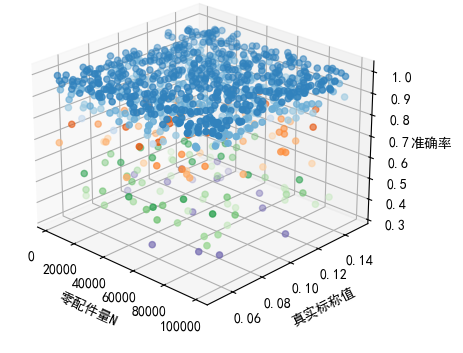
\includegraphics[width=0.48\textwidth]{Fig/Pro1_Accuracy.png}
	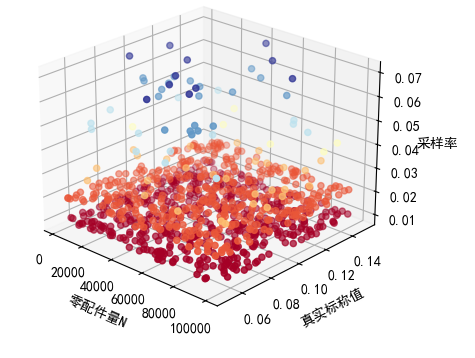
\includegraphics[width=0.48\textwidth]{Fig/Pro1_D.png}

	\begin{minipage}[b]{0.48\textwidth}
		\centering
		(a) 策略采样准确率
	\end{minipage}
	\begin{minipage}[b]{0.48\textwidth}
		\centering
		(b) 策略采样量占比
	\end{minipage}
	\caption{策略采样结果}
	\label{Pro1_result}
\end{figure}
具体来说,我们在$N$和真实标称值的预测范围内均匀采样;对于每个样本点,我们模拟100种样本集情况(这体现在零配件次品的分布次序上);在100种样本集中
由于$N$固定,我们拟合的$\Delta \mu$也固定,因此$SPRT$策略也是固定的,我们充分评估此基准上的假设判断成功率,发现在绝大多数情况下我们的策略都具备
80\%以上的成功率;由于总样本量的跨度较大,我们用策略共采集的样本量在总样本中的占比作为衡量指标,我们的采样占比绝大多数情况小于3\%,这充分体现了
我们采样策略的高效。此外根据我国工业检测国标:对于一般工业零件需要达到2\%-5\%的抽检率\cite{GB/T2828.1-2012},对于高风险零件需要达到10\%以上的抽检率;我们的采样策略是
合乎标准且稳健的。
\section{问题二的模型建立与求解}
首先,我们可以将电子产品加工过程分为三个阶段,即:零配件、成品、市场。每当生产过程从一个阶段进入到另一个阶段均需要决策是否需要
进行抽检,将此过程抽象为图\ref{fig:pro2}。
\begin{figure}[H]
	\centering
	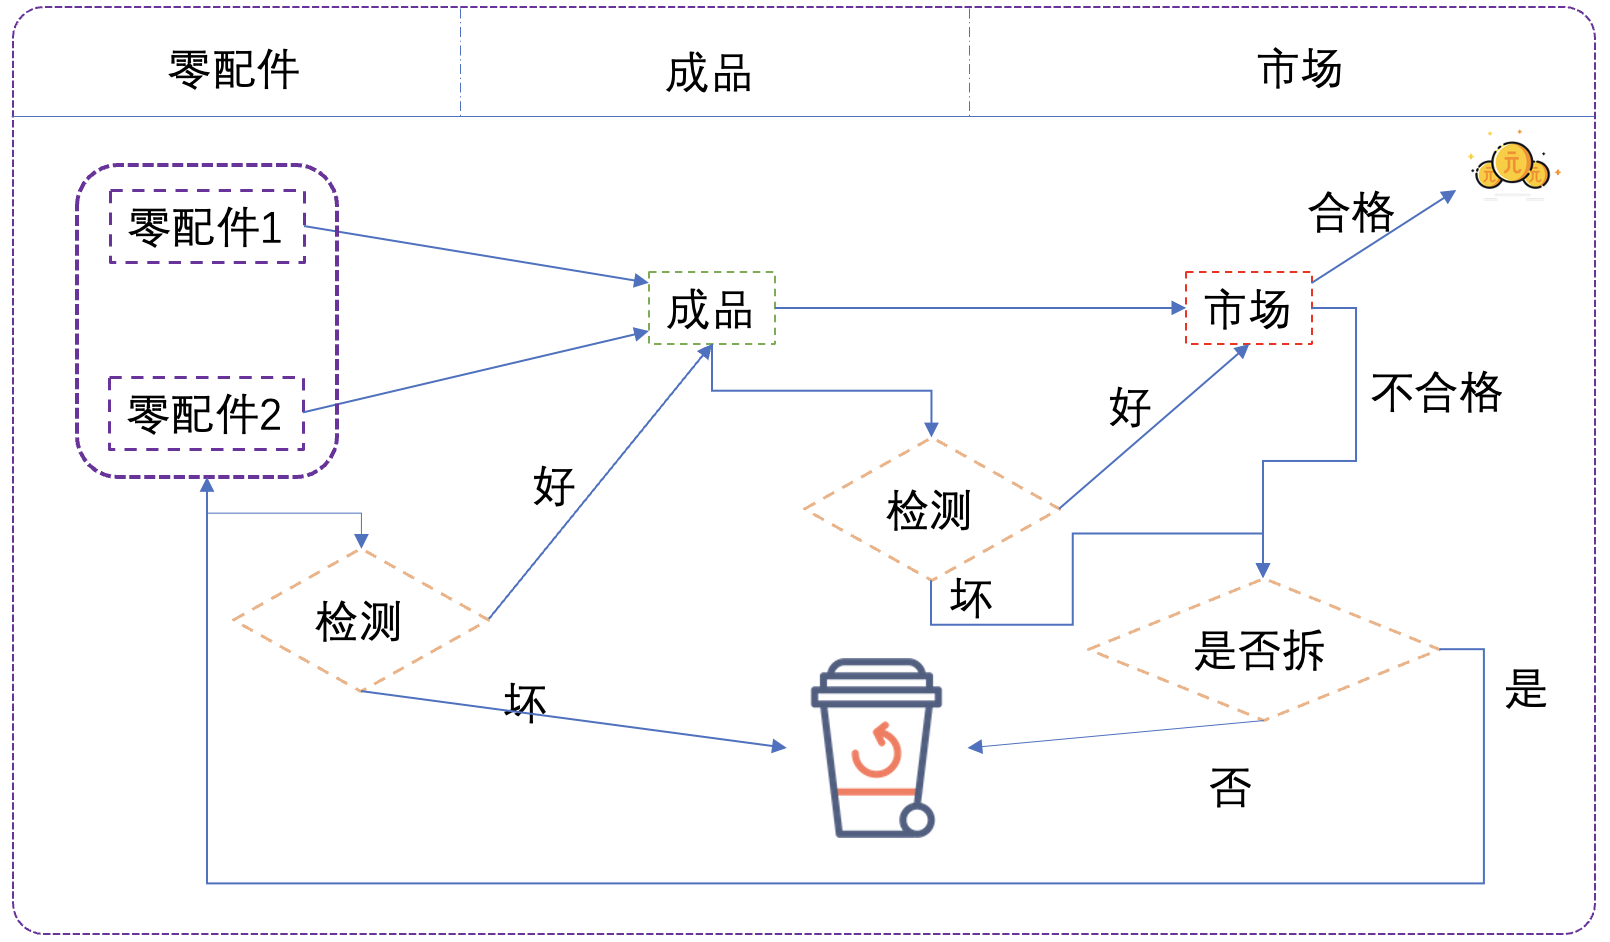
\includegraphics[width=0.8\textwidth,height = 0.4\textwidth]{Fig/pro2.png}      %获得的图片花括号中的名称为figure文件夹中重命名后的图片
	\caption{电子器件生产的流程图}
	\label{fig:pro2}
\end{figure}
在生产流程建模中,我们引入一个决策向量 $\vec{C}=(c_{1},c_{2},c_{3},c_{4})^{T}$,其中每个元素 $c_i$ 分别代表对零配件1、零配件2、成品进行抽样检测,
以及对检测出不合格的成品进行拆解的决策。具体而言,当 $c_{i}$ 取值为0时,表示不进行抽样检测/拆解(丢弃),
而当 $c_{i}$ 取值为1时,表示进行抽样检测/拆解。本文的目标是寻求最优的决策方案 $\vec{C}$,使得生产流程的预期净利润最大化。

由于零部件和成品的次品率均为已知,且假设每批零部件数量 $N$ 充足,我们可以通过排列组合的方式计算出成品中包含不同数量正次品零部件的概率。
假设每批投入的零部件1和零部件2的数量分别为 $N_{1}$ 和 $N_{2}$(其中 $N$ 足够大),且它们的次品率分别为 $\mu_{1}$ 和 $\mu_{2}$。
根据大数定律,我们可以近似认为供应商提供的零部件1和零部件2的次品数量分别为 $N_{1}\cdot\mu_{1}$ 和 $N_{2}\cdot\mu_{2}$。
首先,我们考虑一种简化场景,即不对零部件进行检测,直接将它们组装成成品,且不对不合格成品进行拆解,此时决策向量为 $\vec{C}=(0,0,0,0)^{T}$。
在这种情况下,包含至少一个次品零部件的成品数量 $k$ 的取值范围为 $[\max {N_{1}\cdot\mu_{1},N_{2}\cdot\mu_{2} },N_{1}\cdot\mu_{1}+N_{2}\cdot\mu_{2}]$。
假设在 $k$ 个成品中,分别有 $i$ 个和 $j$ 个零部件1和零部件2为次品,则可知成品中包含 $i$ 个次品零部件1和 $j$ 个次品零部件2的概率 $P_{i,j}$:
\begin{equation}
	P_{i,j}=C_{N_{1}\cdot\mu_{1}}^{i}C_{N_{2}\cdot\mu_{2}}^{j}\mu_{1}^{i}\mu_{2}^{j}(1-\mu_{1})^{k-i}(1-\mu_{2})^{k-j}
	\label{eq:1}
\end{equation}
则$i$和$j$应当满足$i+j\ge k,i\le k,j\le k$,经过计算得到i和j的取值范围为$[k-j,k]$和$[\frac{k}{2},k]$。
我们假设$P_{k}$为存在次品零部件的成品数目为$k$的概率,计算公式如下:
\begin{equation}
	P_{k}=\sum_{i=k-j}^{k}\sum_{j=\frac{k}{2}}^{k}C_{N_{1}\cdot\mu_{1}}^{i}C_{N_{2}\cdot\mu_{2}}^{j}\mu_{1}^{i}\mu_{2}^{j}(1-\mu_{1})^{k-i}(1-\mu_{2})^{k-j}
	\label{eq:2}
\end{equation}
由此可以得到成品中的不合格产品的期望值$M$为($\mu_{3}$为成品次品率):
\begin{equation}
	M=\sum_{k=\max \{N_{1}\cdot\mu_{1},N_{2}\cdot\mu_{2} \}}^{N_{1}\cdot\mu_{1}+N_{2}\cdot\mu_{2}}k\cdot P_{k} + (\min \{ N1,N2\}-k)\cdot \mu_{3}\\
	\label{eq:3}
\end{equation}
令:产品售价为$p_{1}$检测零配件1、2及成品的费用分别为$f_{1}$、$f_{2}$和$f_{3}$,$f_{4}$和$f_{5}$为调换损失及拆解费用,则可以构造产生费用的行向量$\vec{F}=[N_{1}\cdot f_{1},N_{2}\cdot f_{2},\min \{N_{1},N_{2}\}\cdot f_{3},M\cdot f_{5}]$
,考虑产品在上一轮需要退换,我们设置$M^{-1}$为上一轮需要退换产品数(第一轮中$M^{-1}=0$)。
则可以定义本轮零部件池中真实次品率为$\nu_{i}=\frac{M^{-1}+N_{i}\mu_{i}}{M^{-1}+N_{i}}$,其中$i=1,2$。
同时需要计算零配件成本及装配成本,设零配件1、2的成本分别为$d_{1}$、$d_{2}$,装配成本为$d_{3}$,
则可以算出本轮生产的成本函数$cost=d_{1}\cdot N_{1}+d_{2}\cdot N_{2}+\min \{ N_{1},N_{2}\}\cdot d_{3}$,
于是可以将本轮产生的抽检退换费用定义为$R=\vec{F}\cdot\vec{C}+M\cdot f_{4}\cdot c_{3}$
由此能够得到此轮次获利$Profit$:
\begin{equation}
	\textit{Profit}=(\min \{N_{1},N_{2}\}-M^{-1})\cdot p_{1}-R-cost
	\label{eq:4}
\end{equation}
使函数适配16中不同的决策方案,我们需要定义每轮零配件池中所含数量$N'_{1}$、$N'_{2}$即包含每轮次固定补充数量$N_{1}$、$N_{2}$也包含上一轮次零产品拆解后补进的配件(即:$N'=N+M^{-1}\cdot c_{3}$)。
$M$为新轮次中成品次品数目。则零配件池中为次品的平配件数目$n_{1}$、$n_{2}$的计算公式如下:
\begin{equation}
	n_{1}=N_{1}\cdot \mu_{1}+\sum_{j=\frac{k}{2}}^{k}M\cdot P_{i,j} \qquad
	n_{2}=N_{2}\cdot \mu_{2}+\sum_{i=\frac{k}{2}}^{k}M\cdot P_{i,j}
\end{equation}
在此基础上我们可以构造每轮次的收益$Profit$:
\begin{equation}
	\left\{\begin{matrix}
		\textit{Profit}=(\min \{N'_{1}-n_{1}\cdot c_{1},N'_{2}-n_{2}\cdot c_{2}\}-M'\cdot c_{3})\cdot p_{1}-R-cost \\
		M=\sum_{k=\max \{n_{1},n_{2}\}}^{n_{1}+n_{2}}k\cdot P_{k} + (\min \{N'_{1}-n_{1}\cdot c_{1},N'_{2}-n_{2}\cdot c_{2}\}-k)\cdot \mu_{3}\\
	\end{matrix}\right.
	\label{eq:5}
\end{equation}
为了更直观的得到不同决策向量对电子产品生产的收益的影响,我们将图\ref{fig:pro2}中的单次生产流程抽象为一个生产轮次。在每个轮次中我们假设每轮
接受供应商提供的配件数目为固定的$N_{1}$、$N_{2}$,经过上一轮被检测为次品的零部件全部被舍弃,被拆解的成品中的零配件投入下一轮次的零配件池进入生产。
在每轮次生产中我们需要确定不同决策向量以保证电子产品生产的收益,于是我们拟定$t$个生产轮次($t$足够大),每个生产轮次中决策向量$\vec{C}=(c_{1},c_{2},c_{3},c_{4})^{T}$
以此来迭代检验各决策的优劣,如图\ref{fig:pro2-2}。
\begin{figure}[H]
	\centering
	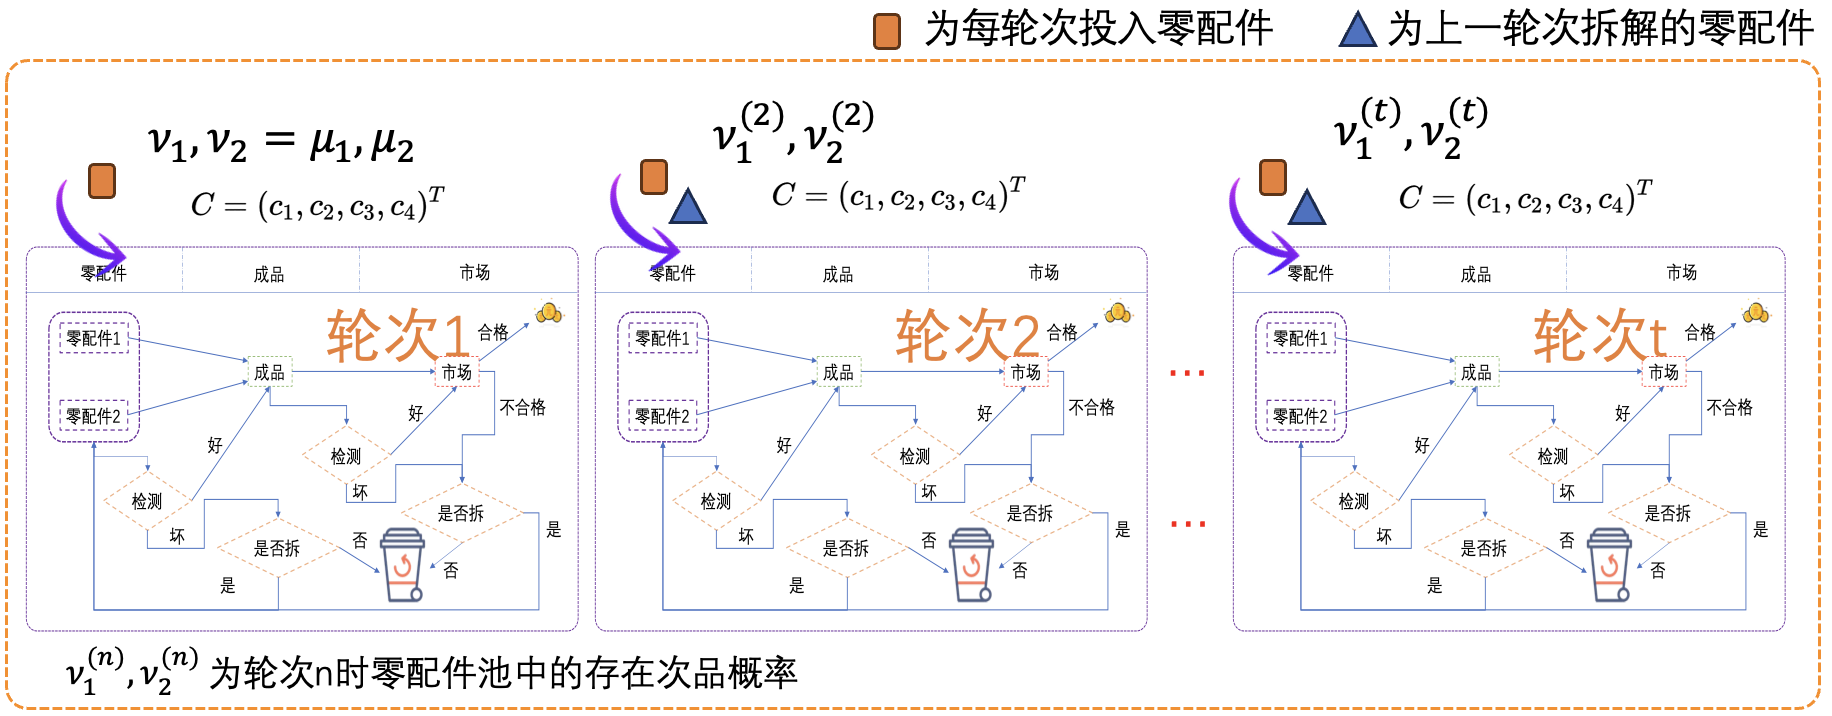
\includegraphics[width=0.85\textwidth]{Fig/pro2-2.png}
	\caption{产品次品率迭代流程图}
	\label{fig:pro2-2}
\end{figure}
综上我们构建了一个以最大获利期望为目标函数的生产的决策模型:
$$	\max \textit{Profit}=\mathbb{E}((\min \{N'_{1}-n_{1}\cdot c_{1},N'_{2}-n_{2}\cdot c_{2}\}-M'\cdot c_{3})\cdot p_{1}-R-cost )\\$$
\begin{equation*}
	s.t.\begin{cases}
		M=\sum_{k=\max \{n_{1},n_{2}\}}^{n_{1}+n_{2}}k\cdot P_{k} + (\min \{N'_{1}-n_{1}\cdot c_{1},N'_{2}-n_{2}\cdot c_{2}\}-k)\cdot \mu_{3}                              \\
		n_{1}=N_{1}\cdot \mu_{1}+\sum_{j=\frac{k}{2}}^{k}M\cdot P_{i,j} \quad n_{2}=N_{2}\cdot \mu_{2}+\sum_{i=\frac{k}{2}}^{k}M\cdot P_{i,j}                                                    \\
		N'_{1}=N_{1}+M^{-1}\cdot c_{3} ,\qquad N'_{2}=N_{2}+M^{-1}\cdot c_{3}                                                                                                                                             \\
		\vec{C}=(c_{1},c_{2},c_{3},c_{4})                                                                                                                                                 \\
		\vec{F}=[N_{1}\cdot f_{1},N_{2}\cdot f_{2},\min \{N_{1},N_{2}\}\cdot f_{3},M\cdot f_{5}]                                                                                         \\
		P_{k}=\sum_{i=k-j}^{k}\sum_{j=\frac{k}{2}}^{k}C_{n_{1}}^{i}C_{n_{2}}^{j}\nu_{1}^{i}\nu_{2}^{j}(1-\nu_{1})^{k-i}(1-\nu_{2})^{k-j}                               \\
		P_{i,j}=C_{n_{1}}^{i}C_{n_{2}}^{j}\nu_{1}^{i}\nu_{2}^{j}(1-\nu_{1})^{k-i}(1-\nu_{2})^{k-j}     \\
		cost=d_{1}\cdot N_{1}+d_{2}\cdot N_{2}+\min \{ N_{1},N_{2}\}\cdot d_{3}
	\end{cases}
\end{equation*}
通过编写求解代码,穷举出所有决策向量$\vec{C}$可能,并且在6个不同情况下计算出每个决策向量的收益期望,最终分别选出最大收益的决策向量$\vec{C}$,作为最优决策方案。
其中0代表不抽检/不拆解,1代表抽检/拆解。
\begin{longtable}{m{1.5cm}<{\centering}ccm{1.5cm}<{\centering}m{1.5cm}<{\centering}c}
	\caption{决策结果图}
	\label{tab:my-table}                    \\
	\hline
	情况 & 零配件1 & 零配件2 & 成品 & 拆解 & 最大纯利润(元/件) \\ \hline
	\endfirsthead
	%
	\endhead
	%
	\hline
	\endfoot
	%
	\endlastfoot
	%
	1  & 1    & 1    & 0  & 1  & 15.83      \\
	2  & 1    & 1    & 0  & 1  & 8.65       \\
	3  & 1    & 1    & 0  & 1  & 13.46      \\
	4  & 1    & 1    & 1  & 1  & 11.33      \\
	5  & 0    & 1    & 0  & 0  & 7.12      \\
	6  & 0    & 0    & 0  & 0  & 18.67     \\ \hline
\end{longtable}
根据结果表\ref{tab:my-table}中结果显示,我们通过对比情况1,2,3得知在零配件和成品的次品率相同时,次品率对最大纯利润的影响远远大于调换损失
的影响,对比情况2和4,在次品率相同的情况下,产品检测成本的降低比调换损失的增加影响更显著,由此证明了此决策方案在零配件次品率较小,检测成本较低的情况下具有较好的稳健性。
情况5更加证实了次品率和抽检成本是影响最大纯利润的关键因素,而非拆解、调换成本,进一步证实了我们决策方案能够将影响利润的因素缩小到可控范围,而对环境
外部因素造成的调换、拆解因素敏感性较低。
在情况6中,我们发现不抽检不拆解的决策方案在纯利润上具有较大优势,这是由于在次品率非常低的情况下,即使不抽检或回收零件都能够保证产品的质量,获得最大的收益。

\section{问题三的模型建立与求解}
首先沿用问题二的思路我们将生产加工过程分为四个阶段,即:零配件准备、半成品、成品、市场。每个阶段都需要决策出抽检方案,此过程可抽象为图\ref{fig:pro3-1}。
\begin{figure}[H]
	\centering
	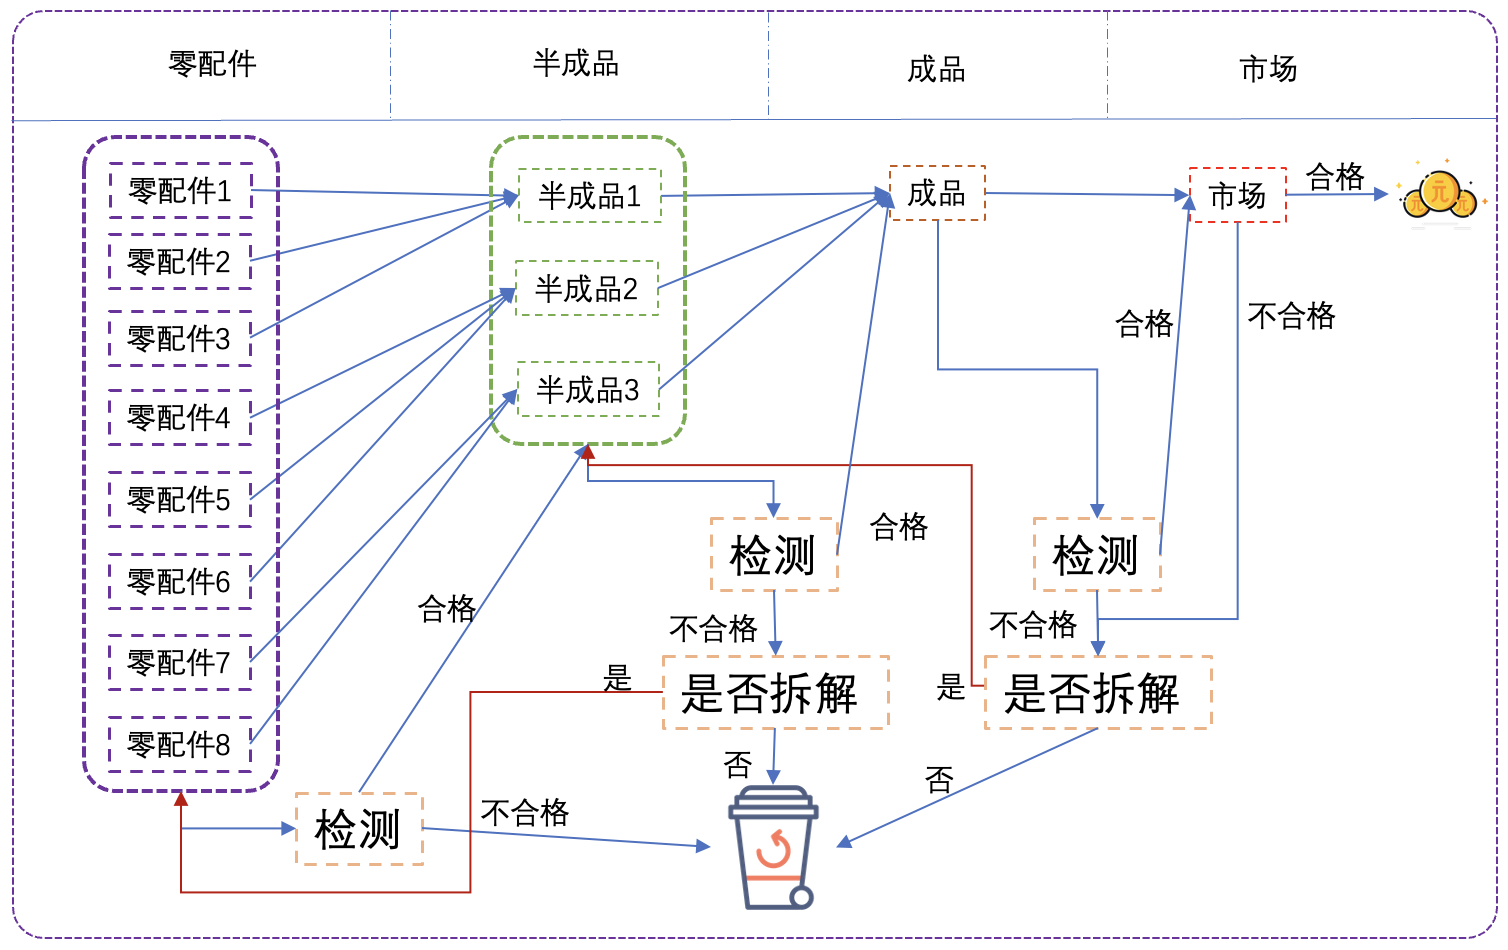
\includegraphics[width=0.8\textwidth]{Fig/pro3-1.png}
	\caption{电子器件生产四阶段的流程图}
	\label{fig:pro3-1}
\end{figure}
对于多个生产阶段的情况中我们设定所有的退货产品如果需要拆解则拆解为半成品,半成品拆解为零配件,然后将生产部件分别投入下一轮次的配件池和半成品池。
题目中要考虑推广到$m$道工序$n$个零配件的情况,我们可以将问题二的模型进行推广,构造决策向量为$\vec{C}=(c_{1},c_{2},\dots,c_{16})^{T}$,其中的元素$c_i$分别表示
零配件1$\sim$8是否抽检、半成品1$\sim$3的抽检和拆解情况以及成品是否抽检、是否拆解($c_{i}$的值为0时表示为不抽检/不拆解(丢弃),值为1时表示检测/拆解)。
我们首先考虑对所有零配件、半成品、成品不进行检测不拆除的情况,即$\vec{C}=(0,0,\dots,0)^{T}$。这里假设半成品中存在次品零部件的半成品数目分别为$k_{1}$、$k_{2}$、$k_{3}$,
成品中存在次品零部件的成品数目为$k$。令8种零配件的次品率为$\mu_{1}$、$\mu_{2}$、$\dots$、$\mu_{8}$,半成品的次品率为$\mu'_{1}$、$\mu'_{2}$、$\mu'_{3}$,成品的次品率为$\mu''$。
与第二问相同我们假定每一轮次投入的零配件数是固定的数值$N_{1}$、$N_{2}$、$\dots$、$N_{8}$,则能够计算出零配件中存在次品的数目为$n_{1}$$\sim$$n_{8}$,其中$n_{i}=N_{i}\cdot\mu_{i}$
		我么设置零配件池中的真实次品占比为$\nu_{1,1},\nu_{1,2},\dots,\nu_{1,8}$(在第一代时$\nu_{1,i}=\mu_{i}$)$\nu_{1,i}=\frac{M_{i}^{-1}\cdot c+N_{i}\mu_{i}}{M_{i}^{-1}\cdot c+N_{i}}$
这里我们用$M^{-1}$来表示上一轮退换回的产品数(第一轮里面$M^{-1}=0$)
以第一个半成品为例,可以得到存在次品零部件的半成品数目为$k_{1}$的概率$P_{k_{1}}$为:
\begin{equation}
	P_{k_{1}}=\sum_{i}\sum_{j}\sum_{z}C_{n_{1}}^{i}C_{n_{2}}^{j}C_{n_{3}}^{z}\nu_{1,1}^{i}\nu_{1,2}^{j}\nu_{1,3}^{z}(1-\nu_{1,1})^{k_{1}-i}(1-\nu_{1,2})^{k_{1}-j}(1-\nu_{1,3})^{k_{1}-z}
	\label{eq:6}
\end{equation}
其中$k_{1}$个半成品中存在的三个零配件情况为$i$、$j$、$z$,则需要满足$i+j+z \ge k_{1}$,$i\le k_{1}$,$j\le k_{1}$,$z\le k_{1}$。
由此能够算出半成品1中不合格品的期望值$M_{1}$为:
\begin{equation}
	M_{1}=\sum_{k_{1}=\max \{n_{1},n_{2},n_{3}\}}^{n_{1}+n_{2}+n_{3}}k_{1}\cdot P_{k_{1}}+(\min \{N_{1},N_{2},N_{3}\}-k_{1})\cdot \mu'_{1}
	\label{eq:7}
\end{equation}
同理可以得到半成品2、半成品3和成品的不合格品的期望值$M_{2}$、$M_{3}$:
\begin{align}
	M_{2} & =\sum_{k_{2}=\max \{n_{4},n_{5},n_{6}\}}^{n_{4}+n_{5}+n_{6}}k_{2}\cdot P_{k_{2}}+(\min \{N_{4},N_{5},N_{6}\}-k_{2})\cdot \mu'_{2} \\
	M_{3} & =\sum_{k_{3}=\max \{n_{7},n_{8}\}}^{n_{7}+n_{8}}k_{3}\cdot P_{k_{3}}+(\min \{N_{7},N_{8}\}-k_{3})\cdot \mu'_{3}
	\label{eq:8}
\end{align}
接着我们能够通过不合格产品的期望算出各个半成品中存在次品的概率$\nu_{2,i}$为:
$$\nu_{2,1}=\frac{M^{-1}\cdot c_{12}+\min \{ n_{1},n_{2},n_{3}\}}{M^{-1}\cdot c_{12}+\min \{N_{1},N_{2},N_{3}\}}$$
$$\nu_{2,2}=\frac{M^{-1}\cdot c_{12}+\min \{ n_{4},n_{5},n_{6}\}}{M^{-1}\cdot c_{12}+\min \{N_{4},N_{5},N_{6}\}}$$
$$\nu_{2,3}=\frac{M^{-1}\cdot c_{12}+\min \{ n_{7},n_{8}\}}{M^{-1}\cdot c_{12}+\min \{N_{7},N_{8}\}}$$
由此我们能够计算出成品中存在次品零部件的成品数目为$k$的概率$P_{k}$为:
\begin{equation}
	P_{k}=\sum_{i}\sum_{j}\sum_{z}C_{M_{1}}^{i}C_{M_{2}}^{j}C_{M_{3}}^{z}\nu_{2,1}^{i}\nu_{2,2}^{j}\nu_{2,3}^{z}(1-\nu_{2,1})^{k_{1}-i}(1-\nu_{2,2})^{k_{1}-j}(1-\nu_{2,3})^{k_{1}-z}
	\label{eq:9}
\end{equation}
其中$k$个成品中存在的三个次半成品情况为$i$、$j$、$z$,则需要满足$i+j+z \ge k$,$i\le k$,$j\le k$,$z\le k$。
由此能够算出成品中不合格品的期望值$M$为:
\begin{equation}
	M=\sum_{k=\max \{M_{1},M_{2},M_{3}\}}^{M_{1}+M_{2}+M_{3}}k\cdot P_{k}+(\min \{N_{1},N_{2},\dots,N_{8}\}-k)\cdot \mu''
	\label{eq:10}
\end{equation}
在理想情况下,所有的成品都进入市场,此时所产生的检测、退换、拆解费用为$\vec{F}=[N_{1}\cdot f_{1},N_{2}\cdot f_{2},\dots,N_{8}\cdot f_{8},
	\min \{ N_{1},N_{2},N_{3}\}\cdot f_{9},\min \{ N_{4},N_{5},N_{6}\}\cdot f_{10},\min \{ N_{7},N_{8}\}\cdot f_{11},\\
	\min \{N_{1},N_{2},\dots,N_{8}\}\cdot f_{12},M_{1}\cdot f_{13},M_{2}\cdot f_{14},M_{3}\cdot f_{15},M\cdot f_{16}]$,此行向量
中$f_{1}$$\sim$$f_{12}$均为抽样检测所产生的费用,$f_{13}$$\sim$$f_{16}$为次品拆解费用,$f_{16}$为退换产生费用。由此能够算出生产线检测、拆解、退换费$R$为:
\begin{equation}
	R=\vec{F}\cdot \vec{C} + M\cdot f_{17}
	\label{eq:11}
\end{equation}
每个阶段所产生的成本可以用$d_{i}\cdot N_{i}$来表示,其中$d_{i}$为每个零配件、半成品、成品的成本费用$i=1,2,\dots,12$,则单轮次成本$cost = \sum_{i=1}^{12}d_{i}\cdot N_{i}$。
综合考虑我们每轮需要调换上一轮里面次品的产品,而这一部分产品无法获利,这里我们用$M^{-1}$来表示上一轮退换回的产品数(第一轮里面$M^{-1}=0$),于是我们能够得到每轮次的收益$Profit$:
\begin{equation}
	\textit{Profit}=(\min \{N_{1},N_{2},\dots,N_{8}\}-M^{-1})\cdot p_{1}-R-cost
	\label{eq:12}
\end{equation}
与问题二类似构建产品动态生产流程图,因为需要考虑的多维参数,我们拟通过遗传进化算法\cite{GA}帮助快速找到最优的生产决策向量$\vec{C}$。
\begin{figure}[H]
	\centering
	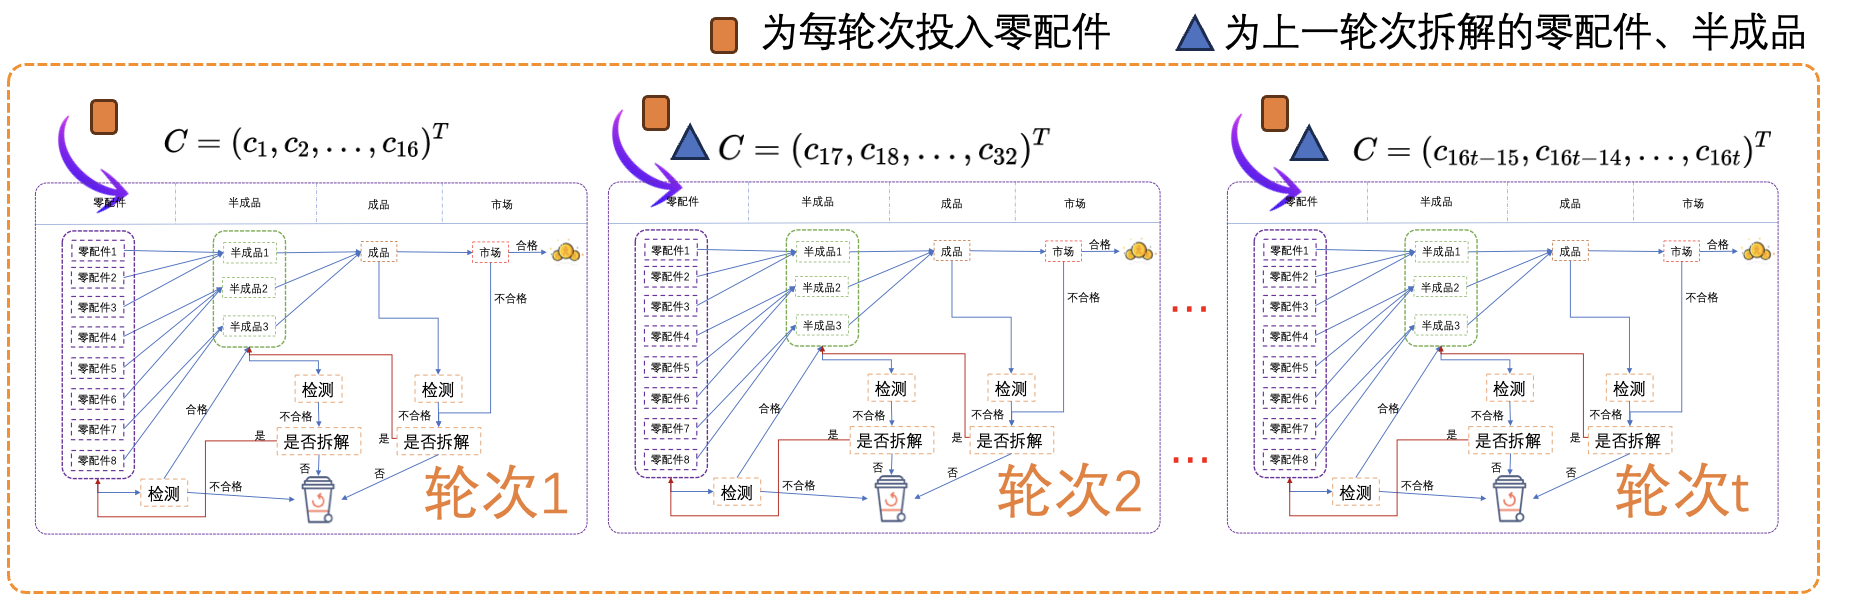
\includegraphics[width=0.8\textwidth]{Fig/pro3-2.png}
	\caption{产品动态生产里路程图图}
	\label{fig:pro3-2}
\end{figure}
综合上述算式,我们能够得到每轮次的收益$Profit$:
$$\max	\textit{Profit}=\mathbb{E}((\min \{N_{1},N_{2},\dots,N_{8}\}-M_{(n)}^{-1})\cdot p_{1}-R-cost)$$
\begin{equation*}
	s.t.\begin{cases}
		R=\vec{F}\cdot \vec{C} + M\cdot f_{17}                                                                                                 \\
		M=\sum_{k=\max \{M_{1},M_{2},M_{3}\}}^{M_{1}+M_{2}+M_{3}}k\cdot P_{k}+(\min \{N_{1},N_{2},\dots,N_{8}\}-k)\cdot \mu''                  \\
		M_{1}=\sum_{k_{1}=\max \{n_{1},n_{2},n_{3}\}}^{n_{1}+n_{2}+n_{3}}k_{1}\cdot P_{k_{1}}+(\min \{N_{1},N_{2},N_{3}\}-k_{1})\cdot \mu'_{1} \\
		M_{2}=\sum_{k_{2}=\max \{n_{4},n_{5},n_{6}\}}^{n_{4}+n_{5}+n_{6}}k_{2}\cdot P_{k_{2}}+(\min \{N_{4},N_{5},N_{6}\}-k_{2})\cdot \mu'_{2} \\
		M_{3}=\sum_{k_{3}=\max \{n_{7},n_{8}\}}^{n_{7}+n_{8}}k_{3}\cdot P_{k_{3}}+(\min \{N_{7},N_{8}\}-k_{3})\cdot \mu'_{3}                   \\
		P_{k_{1}}=\sum_{i}\sum_{j}\sum_{z}C_{n_{1}}^{i}C_{n_{2}}^{j}C_{n_{3}}^{z}\nu_{1,1}^{i}\nu_{1,2}^{j}\nu_{1,3}^{z}(1-\nu_{1,1})^{k_{1}-i}(1-\nu_{1,2})^{k_{1}-j}(1-\nu_{
		1,3})^{k_{1}-z}                                                                                                                        \\
		P_{k_{2}}=\sum_{i}\sum_{j}\sum_{z}C_{n_{4}}^{i}C_{n_{5}}^{j}C_{n_{6}}^{z}\nu_{2,1}^{i}\nu_{2,2}^{j}\nu_{2,3}^{z}(1-\nu_{2,1})^{k_{2}-i}(1-\nu_{2,2})^{k_{2}-j}(1-\nu_{
		2,3})^{k_{2}-z}                                                                                                                        \\
		P_{k_{3}}=\sum_{i}\sum_{j}\sum_{z}C_{n_{7}}^{i}C_{n_{8}}^{j}\nu_{3,1}^{i}\nu_{3,2}^{j}(1-\nu_{3,1})^{k_{3}-i}(1-\nu_{3,2})^{k_{3}-j}   \\
		\nu_{1,i}=\frac{M_{i}^{-1}\cdot c_{j}+N_{i}\mu_{i}}{M_{i}^{-1}\cdot c_{j}+N_{i}} ,i=1\sim8                                                                   \\
\nu_{2,1}=\frac{M^{-1}\cdot c_{15}+\min \{ n_{1},n_{2},n_{3}\}}{M^{-1}\cdot c_{12}+\min \{N_{1},N_{2},N_{3}\}}\quad
\nu_{2,2}=\frac{M^{-1}\cdot c_{15}+\min \{ n_{4},n_{5},n_{6}\}}{M^{-1}\cdot c_{12}+\min \{N_{4},N_{5},N_{6}\}}\quad
\nu_{2,3}=\frac{M^{-1}\cdot c_{15}+\min \{ n_{7},n_{8}\}}{M^{-1}\cdot c_{12}+\min \{N_{7},N_{8}\}}                       \\
		cost = \sum_{i=1}^{8}d_{i}\cdot N_{i}+d_{9}\cdot N_{9}+d_{11}\cdot N_{11}+d_{13}\cdot N_{13}+d_{15}\cdot N_{15}
	\end{cases}
\end{equation*}
与问题二中的求解方法类似,但是因为问题三中的决策向量维度更高,我们需要更加精确的遗传算法来求解最优解,其算法流程如下:

\begin{adjustbox}{width=16cm,height=6.5cm}
    \centering
    \begin{algorithm}[H]
        \SetAlgoLined
        \KwIn{每个阶段决策成本 $Cost_i$, 次品率 $\mu_i$, 变异率 $p_m$, 交叉率 $p_c$, 种群数目 $t$}
        \KwOut{最优决策向量 $\vec{C}^*$, 最大化每轮生产收益 $Profit_{max}$}
        初始化决策向量种群 $P = \{\vec{C}_1, \vec{C}_2, ..., \vec{C}_n\}$, 其中 $\vec{C}_i$ 为随机生成的长度为 $4t$ 的二进制向量 \;
        \While{未达到终止条件}{
            \For{每个个体 $\vec{C}_i \in P$}{
                计算每轮收益 $Profit(\vec{C}_i)$ \;
            }
            计算种群适应度 $Fitness(P)$ \;
            选择父代个体: $Parents \leftarrow Select(P, Fitness(P))$ \;
            \If{$rand() < p_c$}{
                执行交叉操作: $Offspring \leftarrow Crossover(Parents)$ \;
            }
            \If{$rand() < p_m$}{
                执行变异操作: $Offspring \leftarrow Mutate(Offspring)$ \;
            }
            更新种群: $P \leftarrow Update(P, Offspring, Fitness(P \cup Offspring))$ \;
        }
		$\vec{C}^* \leftarrow \underset{\vec{C} \in P}{\operatorname{argmax}}  Profit(\vec{C})$ \;
        $Profit_{max} \leftarrow Profit(\vec{C}^*)$ \;
        \Return $\vec{C}^*, Profit_{max}$
        \caption{遗传算法 (GA) 流程}
    \end{algorithm}
\end{adjustbox}
首先设置合理的变异率、交叉率、种群数目t及各成本参数。通过对随机生成的决策向量进行适应度计算,选择适应度高的个体进行交叉和变异操作,
最后选择最优的个体组成新的种群,直到得到最优决策向量$\vec{C}$为止。我们得到最优的决策向量为$\vec{C}=(1111111100000011)$
,并且最大获利为58.73元/件。此结果表明因为题目中零配件检测单价较低,所以我们选择对8中零配件均进行检测,因而组成半成品的零部件都是
合格品,由此我们不需要对半成品进行检测和拆解,然而考虑到成品的退换成本及零部件成本较高,我们对成品也进行检测并且在检测到次品时进行拆解回收。



\section{问题四的模型建立与求解}
本问题中我们需要考虑到抽样检测的准确性和应对风险的鲁棒性,而不能直接获取真实次品率:相比于对每个阶段的抽样进行风险建模,
一个更为直观的想法是对每一步的预测次品率$\mu$进行概率建模,这样做的好处是便于拟合我们在工序每阶段的概率分布(
这可以被看作是相互独立事件间的概率分布的传播)---我们选用
高斯分布拟合之。事实上,如果我们假定阶段p的期望为问题二及三中给定的次品率,那么:
\begin{equation}
	z_p = \mu_p + \sigma_p \odot \epsilon, \epsilon \sim \mathcal{N}(0, \mathbf{I})
\end{equation}
对于每次评估的$\mu_p$,我们只需计算出相应的风险参数$\sigma_p$,就可以重新从标准高斯分布中采样出噪声施加在其上:
\begin{equation}
	z \sim \mathcal{N}(z; \mu_p, \sigma_p^2 \mathbf{I})
\end{equation}
这样,实际的工序流程中次品率就被建模成了高斯分布,在优化过程中从中采样即可。
\begin{figure}[H]
	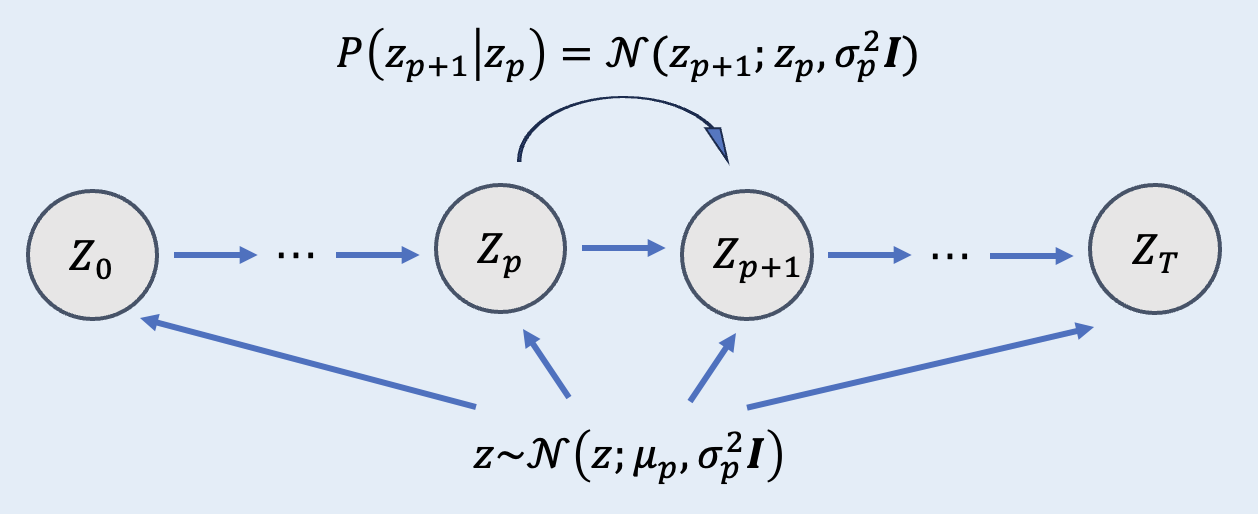
\includegraphics[width=\linewidth]{Fig/pro4.png}
	\caption{工序流程的马尔可夫过程}
	\label{fig:pro4}
\end{figure}
接下来,我们论证该分布在工序流程中的可传播性。
事实上,如果我们把零配件的组装和成品看作一个马尔可夫过程\cite{Markov},如图\ref{fig:pro4},那么,概率分布的传播就可以视为一个前向动力学模型,针对任意的相邻两个工序(
我们暂且搁置对于一般的偏置项的考虑):
\begin{equation}
	\begin{split}
		P(z_{p+1} | z_p) &= \mathcal{N}(z_{p+1};z_p, \sigma_p^2 \mathbf{I}) \\
		&= \mu_{p+1}z_p + \sigma_{p+1} \odot \epsilon \\
		& = \mu_{p+1}(\mu_p + \sigma_p \odot \epsilon) + \sigma_{p+1} \odot \epsilon \\
		& = \mu_{p+1}\mu_p + (\mu_{p+1}\sigma_p + \sigma_{p+1} )\odot \epsilon
	\end{split}
\end{equation}
而又根据独立高斯分布的可加性:$\mathcal{N}(0, \sigma_1^2 \mathbf{I}) + \mathcal{N}(0, \sigma_2^2 \mathbf{I}) \sim \mathcal{N}(0, (\sigma_1^2 + \sigma_2^2) \mathbf{I})$
我们便可以得到$z_{p+1}$的分布:
\begin{equation}
	z_{p+1} \sim \mathcal{N}(z_{p+1}; \mu_{p+1}\mu_p, \sqrt{(\mu_{p+1}\sigma_p)^2 +\sigma_{p+1}^2}\mathbf{I})
\end{equation}
于是,我们的风险就可以通过前向动力学模型来传播了,$\mu$的期望依然遵循于预先设定的标准,而风险可以通过标准差逐层传递\cite{diffusion}。

我们假设对问题二的零配件1,零配件2,成品;问题三的各种零配件,半成品,成品的次品率都采用$SPRT$进行抽样,我们预先设定$H_0$边界范围为:$[S_1,S_2]$;
取其初始值为$\frac{S_1+S_2}{2}$,每次确定其相对预设值的大小后,我们采用二分法逐渐收缩范围,重复10次,设定最终结果为$\mu_i$,并根据与样本集的真实误差
确定$\sigma_i$,在总样本中确定反复取得样本集,获得$\sigma_1,\sigma_2......\sigma_n$,考虑其拟合上文中的高斯分布:
\begin{equation}
	f(x; \sigma_p) = \frac{1}{\sigma_p \sqrt{2\pi}} \exp\left(-\frac{x^2}{2\sigma_p^2}\right)
\end{equation}
观测数据的似然函数是参数 $\sigma_p$ 的函数,它表示在给定参数 $\sigma_p$ 的情况下,观测到数据的概率。由于观测数据独立同分布,因此似然函数可以写成:
\begin{equation}
	L(\sigma_p) = \prod_{i=1}^n f(\sigma_i; \sigma_p) = \prod_{i=1}^n \frac{1}{\sigma_p \sqrt{2\pi}} \exp\left(-\frac{\sigma_i^2}{2\sigma_p^2}\right)
\end{equation}
取其对数似然:
\begin{equation}
	\begin{split}
		\ln L(\sigma_p) &= \sum_{i=1}^n \ln(f(\sigma_i; \sigma_p)) = \sum_{i=1}^n \left[ \ln\left(\frac{1}{\sigma_p \sqrt{2\pi}}\right) - \frac{\sigma_i^2}{2\sigma_p^2} \right] \\
		&= -n \ln(\sigma_p) - n \ln(\sqrt{2\pi}) - \frac{1}{2\sigma_p^2} \sum_{i=1}^n \sigma_i^2
	\end{split}
\end{equation}
求解上述方程,得到参数 $\sigma_p$ 的 MLE\cite{MLE} 估计值:
\begin{equation}
	\hat{\sigma}_p = \sqrt{\frac{\sum_{i=1}^n \sigma_i^2}{n}}
\end{equation}
根据上述的次品率的模型能够算出每个阶段产品的标称值,由此我们给原本各阶段的次品率加上标准差的估计值。
因为标准差的估计是分阶段判断的,现在拟将零配件阶段的,半成品阶段和成品阶段的标准差定位为$\sigma_{1}$,$\sigma_{2}$,$\sigma_{3}$。
则第二问可以将决策方案的目标函数及约束条件改为:
$$	\max \textit{Profit}=\mathbb{E}((\min \{N'_{1}-n_{1}\cdot c_{1},N'_{2}-n_{2}\cdot c_{2}\}-M'\cdot c_{3})\cdot p_{1}-R-cost )\\$$
\begin{equation*}
	s.t.\begin{cases}

		M=\sum_{k=\max \{n_{1},n_{2}\}}^{n_{1}+n_{2}}k\cdot P_{k} + (\min \{N'_{1}-n_{1}\cdot c_{1},N'_{2}-n_{2}\cdot c_{2}\}-k)\cdot \mu_{3}                              \\
		n_{1}=N_{1}\cdot (\mu_{1}+\sigma_{1}\varepsilon)+\sum_{j=\frac{k}{2}}^{k}M\cdot P_{i,j} \quad n_{2}=N_{2}\cdot (\mu_{2}+\sigma_{1}\varepsilon)+\sum_{i=\frac{k}{2}}^{k}M\cdot P_{i,j}                                                    \\
		N'_{1}=N_{1}+M^{-1}\cdot c_{3} ,\qquad N'_{2}=N_{2}+M^{-1}\cdot c_{3}                                                                                                                                             \\
		\vec{C}=(c_{1},c_{2},c_{3},c_{4})                                                                                                                                                 \\
		\vec{F}=[N_{1}\cdot f_{1},N_{2}\cdot f_{2},\min \{N_{1},N_{2}\}\cdot f_{3},M\cdot f_{5}]                                                                                         \\
		P_{k}=\sum_{i=k-j}^{k}\sum_{j=\frac{k}{2}}^{k}C_{n_{1}}^{i}C_{n_{2}}^{j}(\nu_{1}+\sigma_{1}\varepsilon)^{i}(\nu_{2}+\sigma_{2}\varepsilon)^{j}(1-\nu_{1}+\sigma_{1}\varepsilon)^{k-i}(1-\nu_{2}+\sigma_{2}\varepsilon)^{k-j}      \\
		P_{i,j}=C_{n_{1}}^{i}C_{n_{2}}^{j}(\nu_{1}+\sigma_{1}\varepsilon)^{i}(\nu_{2}+\sigma_{2}\varepsilon)^{j}(1-\nu_{1}+\sigma_{1}\varepsilon)^{k-i}(1-\nu_{2}+\sigma_{2}\varepsilon)^{k-j}                                       \\
		cost=d_{1}\cdot N_{1}+d_{2}\cdot N_{2}+\min \{ N_{1},N_{2}\}\cdot d_{3}
	\end{cases}
\end{equation*}
最终结果如表\ref{n_2}所示:
\begin{longtable}{m{1.5cm}<{\centering}ccm{1.5cm}<{\centering}m{1.5cm}<{\centering}c}
    \label{n_2}                             \\
    \hline
    情况 & 零配件1 & 零配件2 & 成品 & 拆解 & 最大纯利润(元/件) \\ \hline
    \endfirsthead
    \endhead
    \hline
    \endfoot
    \endlastfoot
    1  & 1    & 1    & 0  & 1  & 15.55      \\
    2  & 1    & 1    & 0  & 1  & 8.37       \\
    3  & 1    & 1    & 0  & 1  & 13.14      \\
    4  & 1    & 1    & 1  & 1  & 11.03      \\
    5  & 0    & 1    & 0  & 0  & 7.06       \\
    6  & 0    & 0    & 0  & 0  & 18.68      \\ \hline
    \caption{引入误差的决策结果图}
\end{longtable}
我们同样地处理问题三:
$$\max    \sum_{n=1}^{t}\textit{Profit}=(\min \{N_{1},N_{2},\dots,N_{8}\}-M_{(n)}^{-1})\cdot p_{1}-R -cost$$
\begin{equation*}
    s.t.\begin{cases}
        R=\vec{F}\cdot \vec{C} + M\cdot f_{17}                                                                                                 \\
        M=\sum_{k=\max \{M_{1},M_{2},M_{3}\}}^{M_{1}+M_{2}+M_{3}}k\cdot P_{k}+(\min \{N_{1},N_{2},\dots,N_{8}\}-k)\cdot \mu''                  \\
        M_{1}=\sum_{k_{1}=\max \{n_{1},n_{2},n_{3}\}}^{n_{1}+n_{2}+n_{3}}k_{1}\cdot P_{k_{1}}+(\min \{N_{1},N_{2},N_{3}\}-k_{1})\cdot \mu'_{1} \\
        M_{2}=\sum_{k_{2}=\max \{n_{4},n_{5},n_{6}\}}^{n_{4}+n_{5}+n_{6}}k_{2}\cdot P_{k_{2}}+(\min \{N_{4},N_{5},N_{6}\}-k_{2})\cdot \mu'_{2} \\
        M_{3}=\sum_{k_{3}=\max \{n_{7},n_{8}\}}^{n_{7}+n_{8}}k_{3}\cdot P_{k_{3}}+(\min \{N_{7},N_{8}\}-k_{3})\cdot \mu'_{3}                   \\
        P_{k_{1}}=\sum_{i}\sum_{j}\sum_{z}C_{n_{1}}^{i}C_{n_{2}}^{j}C_{n_{3}}^{z}\nu_{1,1}^{i}\nu_{1,2}^{j}\nu_{1,3}^{z}(1-\nu_{1,1})^{k_{1}-i}(1-\nu_{1,2})^{k_{1}-j}(1-\nu_{
        1,3})^{k_{1}-z}                                                                                                                        \\
        P_{k_{2}}=\sum_{i}\sum_{j}\sum_{z}C_{n_{4}}^{i}C_{n_{5}}^{j}C_{n_{6}}^{z}\nu_{2,1}^{i}\nu_{2,2}^{j}\nu_{2,3}^{z}(1-\nu_{2,1})^{k_{2}-i}(1-\nu_{2,2})^{k_{2}-j}(1-\nu_{
        2,3})^{k_{2}-z}                                                                                                                        \\
        P_{k_{3}}=\sum_{i}\sum_{j}\sum_{z}C_{n_{7}}^{i}C_{n_{8}}^{j}\nu_{3,1}^{i}\nu_{3,2}^{j}(1-\nu_{3,1})^{k_{3}-i}(1-\nu_{3,2})^{k_{3}-j}   \\
        \nu_{1,i}=\frac{M_{i}^{-1}+N_{i}(\mu_{i}+\sigma_{i})}{M_{i}^{-1}+N_{i}} ,i=1,2,3                                                       \\
        \nu_{2,i}=\frac{M_{i}^{-1}+\min \{ n_{1},n_{2},n_{3}\}}{M_{i}^{-1}+\min \{N_{1},N_{2},N_{3}\}} i=1,2,3                                 \\
        cost = \sum_{i=1}^{12}d_{i}\cdot N_{i}
    \end{cases}
\end{equation*}
经过求解可以得到最优的决策向量$\vec{C}$与原问题相同,单件最大获利从58.13下降到56.54。

问题二和问题三引入风险后,尽管最优决策向量未发生变化,但单件净利润普遍下降。此现象可由扩散过程中的归纳偏置和风险累计予以解释。
归纳偏置是指模型对未来预测的隐含假设,本文中体现为对每个工序阶段次品率的先验高斯分布假设。此假设引入了认知不确定性,
即对真实次品率的估计存在偏差,该偏差以标准差 $\sigma$ 量化并通过前向扩散过程逐层累加。风险累计是指不确定性在扩散过程中不断累积,导致预测的方差增大,
最终影响净利润期望。具体而言,下一阶段的风险 $\sigma_{p+1}$ 不仅受本阶段风险 $\sigma_p$ 的影响,还受到阶段转移概率 $\mu_{p+1}$ 的放大,
形成类似“滚雪球”效应。因此,即使最优决策向量未变,但由于风险在每个阶段都被放大并传递至下一阶段,最终导致整体净利润期望下降。
此现象也符合信息论哲学,即不确定性的增加必然导致预期收益的减少。

\section{灵敏度分析}
在问题一中,我们考虑$\Delta \mu$的变化对采样准确率和采样量占比的影响。
具体来说,
我们将$\Delta \mu_1,\Delta \mu_2$的值分别向上和向下浮动0-10\%,
同时对$N$的值做出相应浮动以进行测试,在每个测试点,对标称值在5\%-15\%内
均匀采样,最终求得相关指标在各个测试点的均值。
\begin{figure}[htbp]
	\centering
	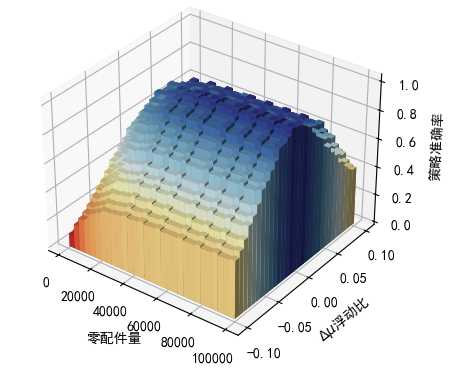
\includegraphics[width=0.48\textwidth]{Fig/pro1_sensi_acc.png}
	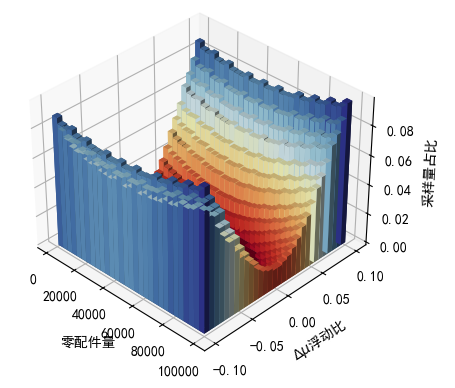
\includegraphics[width=0.48\textwidth]{Fig/pro1_sensi_ocu.png}
	\begin{minipage}[b]{0.48\textwidth}
		\centering
		(a) 采样准确率分析
	\end{minipage}
	\begin{minipage}[b]{0.48\textwidth}
		\centering
		(b) 采样量占比分析
	\end{minipage}
	\caption{\textit{SPRT}灵敏度分析}
	\label{Pro1_sensi}
\end{figure}
可以发现,我们的模型在面对大跨度的样本量时有较强的鲁棒性;针对某一特定的真实次品率,采样量占比和采样准确率对样本量的变化
都不敏感,这充分说明我们的模型能够适应不同的工业生产要求情况。另一方面,考虑到$\Delta \mu$在不同浮动值下模型的表现,我们发现
在两项指标上模型对$\Delta \mu$的浮动都较为敏感。在10\%的浮动率内足以使模型的策略准确率明显降低和采样量显著增大。这证实了该参数
对模型的影响是相当深刻的。在问题一中我们采用未经扰动的,由MLP直接输出的$\Delta \mu$参与$SPRT$抽样时,策略准确率维持在0.8以上的
较高水平,而采样量维持在3\%以下的较低水平。这足以证明MLP对于$\Delta \mu$的拟合相当有效,它的拟合误差在极其小的范围内,因此不会
出现以上浮动所带来的不稳定结果。
\begin{table}[htbp]
    \centering
    \renewcommand\arraystretch{1.0}
    \setlength\tabcolsep{16pt}
    \footnotesize
    \begin{tabular}{c|c|c|c|c|c|c|c}
        \hline
                & \multicolumn{7}{c}{零配件量$N$}                                                 \\
        \cline{2-8}
        工序场景    & 100                         & 200   & 400   & 800   & 1600  & 3200  & 6400  \\
        \hline
        问题2-情况1 & 16.03                       & 15.92 & 15.87 & 15.84 & 15.83 & 15.81 & 15.79 \\
        问题2-情况2 & 8.85                        & 8.74  & 8.69  & 8.66  & 8.63  & 8.62  & 8.61  \\
        问题2-情况3 & 13.87                       & 13.64 & 13.53 & 13.47 & 13.44 & 13.38 & 13.29 \\
        问题2-情况4 & 11.47                       & 11.39 & 11.35 & 11.33 & 11.33 & 11.31 & 11.31 \\
        问题2-情况5 & 7.23                        & 7.17  & 7.14  & 7.07  & 7.05  & 7.07  & 7.05  \\
        问题2-情况6 & 19.02                       & 18.67 & 18.68 & 18.67 & 18.69 & 18.69 & 18.67 \\
        问题3     & 59.26                       & 58.85 & 58.84 & 58.73 & 58.69 & 58.69 & 58.68 \\
        \hline
    \end{tabular}
    \caption{零配件总量变化时不同情况下单件利润}
    \label{pro2_sensi}
\end{table}

为深入探究零部件总量对模型稳健性的影响,我们针对问题二的六种情况和问题3开展了精细化的灵敏度分析,分析结果如表\ref{pro2_sensi}所示。通过对其进行细致分析,
我们观察到模型的决策方案在应对不同零部件总量变化时展现出卓越的稳健性。首先,从宏观层面来看, 尽管所有情况下的单件利润都随着零部件总量的增加呈现出下
降趋势,但值得注意的是,这种下降趋势并非线性关系,而是呈现出一种渐进式下降的趋势,体现了模型决策的精细化和对成本控制的有效性。其次,从微观层面来看,
针对每种场景,单件利润的下降幅度都较为平缓,进一步印证了模型的稳健性。例如,在情况1中,当零部件总量从100增加到6400时,单件利润仅下降了0.24元,
下降幅度仅为初始值的1.5\%;在情况6中,即使零部件总量增加64倍,单件利润也仅仅下降了0.35元,下降幅度仅为初始值的1.8\%。
此外,通过对比不同情况下的下降幅度, 我们发现次品率和产品检测成本对模型稳健性的影响更为显著,而调换损失的影响相对较小。
这表明模型能够有效地应对次品率和产品检测成本的波动,从而保证企业在不同生产环境下都能获得相对稳定的收益。综上所述, 模型的决策方案在面对
不同规模的生产需求时能够保持卓越的适应性和稳定性,体现了模型的鲁棒性,为企业在复杂多变的市场环境中制定科学合理的生产决策提供了有力支撑。

\section{模型评价}
这篇论文针对电子产品生产线的多阶段质量控制问题,提出了一个基于序贯概率比检验 $SPRT$、
优化算法和高斯过程的综合决策模型。其优势主要体现在以下方面:

(1)\textbf{动态抽样策略:} 利用 SPRT 构建了动态调整零部件抽样方案的决策模型。通过引入扰动量,构建零假设和备择假设下的似然函数,并采用多层感知机 $MLP$ 对扰动量进行函数拟合,实现了在低抽样率下对零部件批次做出高精度决策。

(2)\textbf{多阶段策略优化:} 针对多阶段生产流程,构建了多轮次决策向量并通过遗传算法找到最优决策方案。该方法能够有效地处理多阶段、多零部件的复杂生产流程,并最大化生产净利润。

(3)\textbf{误差传递建模:} 将各阶段由于抽样误差所引起的归纳误差建模为马尔可夫过程,并将单次偏差量化高斯分布。通过前向扩散过程论证了误差传递策略的有效性,并利用最大似然估计回归出单次误差分布,使得模型更具鲁棒性。

然而在现实应用中,模型也具有明显的不足之处和可发展性:

\textbf{理想模型的简化性:} 模型假设每批零部件的次品率严格服从二项分布,
并且每次抽检结果为次品的事件之间相互独立。然而,在实际生产过程中,
次品率可能受到多种因素的影响,例如原材料质量、生产工艺、操作人员等,
并且次品事件之间可能存在关联性。这些因素可能导致模型的假设与实际情况存在
偏差,从而影响模型的可靠性。


%参考文献
\begin{thebibliography}{9}%宽度9
	\bibitem[1]{GA}Genetic algorithms, JH Holland - Scientific american, 1992 - JSTOR

	\bibitem[2]{GB/T2828.1-2012}国家标准,
	\textit{计数抽样检验程序 第1部分:按接收质量限(AQL)检索的逐批检验抽样计划 (GB/T 2828.1-2012)}. 中国标准出版社.

	\bibitem[3]{diffusion}The solution-diffusion model: a review, JG Wijmans, RW Baker - Journal of membrane science

	\bibitem[4]{Markov}Markov processes, EB Dynkin, EB Dynkin - 1965 - Springer

	\bibitem[5]{Approximation}Approximation theory of the MLP model in neural networks, A Pinkus - Acta numerica, 1999 - cambridge.org

	\bibitem[6]{MLE}The MLE algorithm for the matrix normal distribution,P Dutilleul - Journal of statistical computation and simulation, 1999 - Taylor \& Francis

	\bibitem[7]{SPRT}Optimum character of the sequential probability ratio test, A Wald, J Wolfowitz - The Annals of Mathematical Statistics, 1948 - JSTOR
\end{thebibliography}

\newpage
%附录
\subsection{附录参考说明}
支撑材料文件目录:
\begin{itemize}
	\item \textbf{sprt.py} ——SPRT算法源程序(问题一)
	\item \textbf{pro1\_sensi.py} ——问题一灵敏度分析源程序
	\item \textbf{2\_1.py} ——问题二方案一源程序
	\item \textbf{2\_2.py} ——问题二方案二源程序
	\item \textbf{2\_3.py} ——问题二方案三源程序
	\item \textbf{2\_4.py} ——问题二方案四源程序
	\item \textbf{2\_5.py} ——问题二方案五源程序
	\item \textbf{2\_6.py} ——问题二方案六源程序
	\item \textbf{Question\_3.py} ——问题三源程序
	\item \textbf{4\_2\_1.py} ——问题四针对问题二方案一源程序
	\item \textbf{4\_2\_2.py} ——问题四针对问题二方案二源程序
	\item \textbf{4\_2\_3.py} ——问题四针对问题二方案三源程序
	\item \textbf{4\_2\_4.py} ——问题四针对问题二方案四源程序
	\item \textbf{4\_2\_5.py} ——问题四针对问题二方案五源程序
	\item \textbf{4\_2\_6.py} ——问题四针对问题二方案六源程序
	\item \textbf{4\_3.py} ——问题四针对问题三源程序
	\item \textbf{gaussion.py} ——问题四高斯分布源程序
\end{itemize}
\begin{appendices}
	\section{问题一的Python代码}
\subsection{pro1\_sensi.py(第一问灵敏度分析代码)}
	\begin{lstlisting}[language=python]
		import torch
		import torch.nn as nn
		import torch.optim as optim
		import numpy as np
		from tqdm import tqdm
		
		class MLP(nn.Module):
			def __init__(self, input_size, hidden_size, output_size):
				super(MLP, self).__init__()
				self.fc1 = nn.Linear(input_size, hidden_size[0])
				self.relu1 = nn.ReLU()
				self.fc2 = nn.Linear(hidden_size[0], hidden_size[1])
				self.relu2 = nn.ReLU()
				self.fc3 = nn.Linear(hidden_size[1], output_size)
		
			def forward(self, x):
				x = self.fc1(x)
				x = self.relu1(x)
				x = self.fc2(x)
				x = self.relu2(x)
				x = self.fc3(x)
				return x
		
		def SPRT(S, delta_mu, alpha=0.05, beta=0.1):
			A = torch.tensor(np.log((1 - beta) / alpha), dtype=torch.float32).to(device)
			B = torch.tensor(np.log(beta / (1 - alpha)), dtype=torch.float32).to(device)
			batch_size = S.shape[0]
			predictions = torch.zeros(batch_size, dtype=torch.float32, requires_grad=True).to(device)
			samples_taken = torch.zeros(batch_size, dtype=torch.float32).to(device)
			for i in range(batch_size):
				sample = S[i]
				D1 = int(0.01 * sample.shape[0]) 
				LR = torch.tensor(0.0, dtype=torch.float32).to(device)
				hint = 1  
		
				j = 1 
				n1 = sample[:D1]
				while True:  
					mu0_pred = torch.tensor(0.1, dtype=torch.float32).to(device) + delta_mu[0]
					mu1_pred = torch.tensor(0.1, dtype=torch.float32).to(device) - delta_mu[1]
					LR_numerator = torch.sum(n1 * torch.log(mu0_pred) + (1 - n1) * torch.log(1 - mu0_pred))
					LR_denominator = torch.sum(n1 * torch.log(mu1_pred) + (1 - n1) * torch.log(1 - mu1_pred))
					LR = LR_numerator / (LR_denominator + 1e-19)
		
					if LR <= A:
						hint = 0
						break
					elif LR >= B:
						hint = 1
						break
					else:
						j += 1
						if 2 * D1 - int(torch.sum(n1).item()) >= len(sample):
							break  
						n1 = sample[D1: 2 * D1 - int(torch.sum(n1).item())]
				predictions[i] = hint
				samples_taken[i] = j * D1 
		
			return predictions, samples_taken
		
		def train_model(model, optimizer, criterion, epoch, epochs, delta_mu):
			model.train()
			running_loss = 0.0
			for i in tqdm(range(10000), ncols=100, desc="Training"):
				N = np.random.randint(1000, 100000)
				gt = np.random.uniform(gt_range[0], gt_range[1])
				sample = np.random.choice([0, 1], size=N, p=[gt, 1 - gt])
				if gt > 0.1:
					gt = 0
				else:
					gt = 1
				inputs = torch.tensor([N], dtype=torch.float32).to(device)
				targets = torch.tensor([gt], dtype=torch.float32).to(device)
				outputs = model(inputs) + torch.tensor(delta_mu, dtype=torch.float32).to(device)
				pred, samples = SPRT(torch.tensor([sample], dtype=torch.float32).to(device), outputs)
				loss = criterion(pred.float(), targets.float())
				loss.backward()
				optimizer.step()
				optimizer.zero_grad()
				running_loss += loss.item()
			return running_loss / 10000
		
		
		def evaluate_model(model, criterion, delta_mu):
			model.eval()
			running_loss = 0.0
			correct = 0
			total = 0
			total_samples = 0
			with torch.no_grad():
				for i in tqdm(range(1000), ncols=100, desc="Evaluating"):
					N = np.random.randint(1000, 100000)
					gt = np.random.uniform(gt_range[0], gt_range[1])
					sample = np.random.choice([0, 1], size=N, p=[gt, 1 - gt])
					if gt > 0.1:
						gt = 0
					else:
						gt = 1
					inputs = torch.tensor([N], dtype=torch.float32).to(device)
					targets = torch.tensor([gt], dtype=torch.float32).to(device)
					outputs = model(inputs) + torch.tensor(delta_mu, dtype=torch.float32).to(device)
					pred, samples = SPRT(torch.tensor([sample], dtype=torch.float32).to(device), outputs)
					loss = criterion(pred.float(), targets.float())
					running_loss += loss.item()
					correct += (pred == targets).sum().item()
					total += 1
					total_samples += samples.item()
			accuracy = correct / total
			average_samples = total_samples / total
			return running_loss / 1000, accuracy, average_samples
		
		
		if __name__ == "__main__":
			gt_range = (0.05, 0.15)
			input_size = 1
			hidden_size = [16, 64]
			output_size = 2
			learning_rate = 0.001
			epochs = 10
			batch_size = 32
			criterion = nn.MSELoss()
			device = torch.device("cuda:0" if torch.cuda.is_available() else "cpu")
		
			# 灵敏度分析:遍历 delta_mu
			delta_mu_values = np.arange(0.01, 0.11, 0.01)  
			results = []
			for delta_mu in delta_mu_values:
				print(f"Evaluating delta_mu = {delta_mu:.2f}")
				
		
				model = MLP(input_size, hidden_size, output_size).to(device)
				optimizer = optim.Adam(model.parameters(), lr=learning_rate)
				
				for epoch in range(epochs):
					train_loss = train_model(model, optimizer, criterion, epoch, epochs, [delta_mu, delta_mu])
					test_loss, accuracy, average_samples = evaluate_model(model, criterion, [delta_mu, delta_mu])
					print(
						f"Epoch {epoch+1}, Train Loss: {train_loss:.4f}, Test Loss: {test_loss:.4f}, "
						f"Accuracy: {accuracy:.4f}, Average Samples: {average_samples:.2f}"
					)
				
				results.append((delta_mu, accuracy, average_samples))
		
			print("\nSensitivity Analysis Results:")
			print("Delta Mu | Accuracy | Average Samples")
			print("----------|----------|----------------")
			for delta_mu, accuracy, average_samples in results:
				print(f"{delta_mu:.2f}       | {accuracy:.4f}   | {average_samples:.2f}")
		
		
	 \end{lstlisting}
\subsection{sprt.py}
	 \begin{lstlisting}[language=python]
		import torch
import torch.nn as nn
import torch.optim as optim
import numpy as np
from tqdm import tqdm  

class MLP(nn.Module):
    def __init__(self, input_size, hidden_size, output_size):
        super(MLP, self).__init__()
        self.fc1 = nn.Linear(input_size, hidden_size[0])
        self.relu1 = nn.ReLU()
        self.fc2 = nn.Linear(hidden_size[0], hidden_size[1])
        self.relu2 = nn.ReLU()
        self.fc3 = nn.Linear(hidden_size[1], output_size)

    def forward(self, x):
        x = self.fc1(x)
        x = self.relu1(x)
        x = self.fc2(x)
        x = self.relu2(x)
        x = self.fc3(x)
        return x

def SPRT(S, delta_mu, alpha=0.05, beta=0.1):
    A = torch.tensor(np.log((1 - beta) / alpha), dtype=torch.float32).to(device)
    B = torch.tensor(np.log(beta / (1 - alpha)), dtype=torch.float32).to(device)
    batch_size = S.shape[0]
    predictions = torch.zeros(batch_size, dtype=torch.float32, requires_grad=True).to(device)
    for i in range(batch_size):
        sample = S[i]
        D1 = int(0.01 * sample.shape[0])  # 初始样本量
        LR = torch.tensor(0.0, dtype=torch.float32).to(device)
        hint = 1  # 初始化预测假设为1

        j = torch.ones(batch_size, dtype=torch.float32, requires_grad=True).to(device)
        n1 = sample[:D1]
        while j < 10:
            mu0_pred = torch.tensor(0.1, dtype=torch.float32).to(device) + delta_mu[0]
            mu1_pred = torch.tensor(0.1, dtype=torch.float32).to(device) - delta_mu[1]
            LR_numerator = torch.sum(n1 * torch.log(mu0_pred) + (1 - n1) * torch.log(1 - mu0_pred))
            LR_denominator = torch.sum(n1 * torch.log(mu1_pred) + (1 - n1) * torch.log(1 - mu1_pred))
            LR = LR_numerator / (LR_denominator + 1e-19)

            if LR <= A:
                hint = 0
                break
            elif LR >= B:
                hint = 1
                break
            else:
                j += 1
                n1 = sample[D1 : 2 * D1 - int(torch.sum(n1).item())]
        predictions[i] = hint

    return predictions,j

def train_model(model, optimizer, criterion, epoch, epochs):
    model.train()
    running_loss = 0.0
    for i in tqdm(range(10000), ncols=100, desc="Training"):
        N = np.random.randint(1000, 100000)
        gt = np.random.uniform(gt_range[0], gt_range[1])
        sample = np.random.choice([0, 1], size=N, p=[gt, 1 - gt])
        if gt > 0.1:
            gt = 0
        else:
            gt = 1
        inputs = torch.tensor([N], dtype=torch.float32).to(device)
        targets = torch.tensor([gt], dtype=torch.float32).to(device)
        outputs = model(inputs)
        pred,j = SPRT(torch.tensor([sample], dtype=torch.float32).to(device), outputs)
        loss = j*criterion(pred.float(), targets.float())
        loss.backward()
        optimizer.step()
        optimizer.zero_grad()
        running_loss += loss.item()
    return running_loss / 10000


def evaluate_model(model, criterion):
    model.eval()
    running_loss = 0.0
    correct = 0
    total = 0
    with torch.no_grad():
        for i in tqdm(range(1000), ncols=100, desc="Evaluating"):
            N = np.random.randint(1000, 100000)
            gt = np.random.uniform(gt_range[0], gt_range[1])
            sample = np.random.choice([0, 1], size=N, p=[gt, 1 - gt])
            if gt > 0.1:
                gt = 0
            else:
                gt = 1
            inputs = torch.tensor([N], dtype=torch.float32).to(device)
            targets = torch.tensor([gt], dtype=torch.float32).to(device)
            outputs = model(inputs)
            pred,_ = SPRT(torch.tensor([sample], dtype=torch.float32).to(device), outputs)
            loss = criterion(pred.float(), targets.float())
            running_loss += loss.item()
            correct += (pred == targets).sum().item()
            total += 1
    accuracy = correct / total
    return running_loss / 1000, accuracy


if __name__ == "__main__":
    gt_range = (0.05, 0.15)
    input_size = 1
    hidden_size = [16, 64]
    output_size = 2
    learning_rate = 0.001
    epochs = 1000
    batch_size = 32

    device = torch.device("cuda:3" if torch.cuda.is_available() else "cpu")

    model = MLP(input_size, hidden_size, output_size).to(device)
    optimizer = optim.Adam(model.parameters(), lr=learning_rate)
    criterion = nn.MSELoss()

    for epoch in range(epochs):
        train_loss = train_model(model, optimizer, criterion, epoch, epochs)
        test_loss, accuracy = evaluate_model(model, criterion)
        print(
            f"Epoch {epoch+1}, Train Loss: {train_loss:.4f}, Test Loss: {test_loss:.4f}, Accuracy: {accuracy:.4f}"
        )

	\end{lstlisting}
\section{问题二的python代码}
\subsection{2\_1.py(决策向量求解)}
\begin{lstlisting}[language=python]
	import random
import numpy as np
from scipy.special import comb

def Solve(Element_S1, Element_S2, Test_Mark_S1, Test_Mark_S2, Test_Mark_Finished_Product, Dismantle_Mark_Finished_Product, Exchange_Quantity):

    Profit = 0
    Cost = 0
    Test_Price_S1 = 2
    Test_Price_S2 = 3
    Finished_Product_Defect_Rate = 0.1
    Finished_Product_Assemble_Price = 6
    Finished_Product_Test_Price = 3
    Finished_Product_Sell_Price = 56
    Finished_Product_Exchange_Loss = 6
    Finished_Product_Dismantle_cost = 5

    # 零件阶段
    if Test_Mark_S1 == 1:
        Cost += Test_Price_S1 * len(Element_S1)
        Element_S1 = [x for x in Element_S1 if x != 0]
    if Test_Mark_S2 == 1:
        Cost += Test_Price_S2 * len(Element_S2)
        Element_S2 = [x for x in Element_S2 if x != 0]

    random.shuffle(Element_S1)
    random.shuffle(Element_S2)

    if len(Element_S1) == len(Element_S2):
        Finished_Product = [int(a * b) for a, b in zip(Element_S1, Element_S2)]
        Finished_Product_Form = np.array([Element_S1, Element_S2])
        Cost += Finished_Product_Assemble_Price * len(Finished_Product)
        Qualified_Finished_Products_Indices = [index for index, value in enumerate(Finished_Product) if value == 1]
        Num_To_Select = int(len(Qualified_Finished_Products_Indices) * Finished_Product_Defect_Rate)
        Qualified_Finished_Products_Selected_Indices = np.random.choice(Qualified_Finished_Products_Indices, size=Num_To_Select, replace=False)
        for index in Qualified_Finished_Products_Selected_Indices:
            Finished_Product[index] = 0
        Element_S1 = []
        Element_S2 = []
    elif len(Element_S1) < len(Element_S2):
        Selected_Indices_S2 = random.sample(range(len(Element_S2)), len(Element_S1))
        Selected_Element_S2 = [Element_S2[i] for i in Selected_Indices_S2]
        Finished_Product = [int(a * b) for a, b in zip(Element_S1, Selected_Element_S2)]
        Finished_Product_Form = np.array([Element_S1, Selected_Element_S2])
        Cost += Finished_Product_Assemble_Price * len(Finished_Product)
        Qualified_Finished_Products_Indices = [index for index, value in enumerate(Finished_Product) if value == 1]
        Num_To_Select = int(len(Qualified_Finished_Products_Indices) * Finished_Product_Defect_Rate)
        Qualified_Finished_Products_Selected_Indices = np.random.choice(Qualified_Finished_Products_Indices, size=Num_To_Select, replace=False)
        for index in Qualified_Finished_Products_Selected_Indices:
            Finished_Product[index] = 0
        Element_S1 = []
        Element_S2 = [Element_S2[i] for i in range(len(Element_S2)) if i not in Selected_Indices_S2]
    elif len(Element_S1) > len(Element_S2):
        Selected_Indices_S1 = random.sample(range(len(Element_S1)), len(Element_S2))
        Selected_Element_S1 = [Element_S1[i] for i in Selected_Indices_S1]
        Finished_Product = [int(a * b) for a, b in zip(Selected_Element_S1, Element_S2)]
        Finished_Product_Form = np.array([Selected_Element_S1, Element_S2])
        Cost += Finished_Product_Assemble_Price * len(Finished_Product)
        Qualified_Finished_Products_Indices = [index for index, value in enumerate(Finished_Product) if value == 1]
        Num_To_Select = int(len(Qualified_Finished_Products_Indices) * Finished_Product_Defect_Rate)
        Qualified_Finished_Products_Selected_Indices = np.random.choice(Qualified_Finished_Products_Indices, size=Num_To_Select, replace=False)
        for index in Qualified_Finished_Products_Selected_Indices:
            Finished_Product[index] = 0
        Element_S1 = [Element_S1[i] for i in range(len(Element_S1)) if i not in Selected_Indices_S1]
        Element_S2 = []

    # 成品阶段
    if Test_Mark_Finished_Product == 1:
        Cost += Finished_Product_Test_Price * len(Finished_Product)
        Qualified_Finished_Products_Indices = [index for index, value in enumerate(Finished_Product) if value == 1]
        Unqualified_Finished_Products_Indices = [index for index, value in enumerate(Finished_Product) if value == 0]
        Profit += Finished_Product_Sell_Price * (len(Qualified_Finished_Products_Indices) - Exchange_Quantity)
        Exchange_Quantity = 0
        if Dismantle_Mark_Finished_Product == 1:
            Cost += Finished_Product_Dismantle_cost * len(Unqualified_Finished_Products_Indices)
            Unqualified_Finished_Product_Form = Finished_Product_Form[:, Unqualified_Finished_Products_Indices]
            Element_S1.extend(Unqualified_Finished_Product_Form[0])
            Element_S2.extend(Unqualified_Finished_Product_Form[1])
    else:
        Qualified_Finished_Products_Indices = [index for index, value in enumerate(Finished_Product) if value == 1]
        Unqualified_Finished_Products_Indices = [index for index, value in enumerate(Finished_Product) if value == 0]
        Profit += Finished_Product_Sell_Price * (len(Finished_Product) - Exchange_Quantity)
        Exchange_Quantity = 0
        Cost += Finished_Product_Exchange_Loss * len(Unqualified_Finished_Products_Indices)
        Exchange_Quantity = len(Unqualified_Finished_Products_Indices)
        if Dismantle_Mark_Finished_Product == 1:
            Cost += Finished_Product_Dismantle_cost * len(Unqualified_Finished_Products_Indices)
            Unqualified_Finished_Product_Form = Finished_Product_Form[:, Unqualified_Finished_Products_Indices]
            Element_S1.extend(Unqualified_Finished_Product_Form[0])
            Element_S2.extend(Unqualified_Finished_Product_Form[1])

    return Profit, Cost, Element_S1, Element_S2, Exchange_Quantity

S1 = S2 = 1000
Defect_Rate_S1 = 0.1
Defect_Rate_S2 = 0.1
Bad_S1 = int(Defect_Rate_S1 * S1)
Bad_S2 = int(Defect_Rate_S2 * S2)

Time = 1
Simulation_Number = 100
Profits = np.zeros(16)
Costs = np.zeros(16)
Purchase_Price_S1 = 4
Purchase_Price_S2 = 18

Decision_Matrix = np.zeros((16, 4), dtype=int)
for i in range(16):
    Binary_Representation = format(i, '04b')
    for j in range(4):
        Decision_Matrix[i, j] = int(Binary_Representation[j])

for i in range(0,16):
    Test_Mark_S1 = Decision_Matrix[i][0]
    Test_Mark_S2 = Decision_Matrix[i][1]
    Test_Mark_Finished_Product = Decision_Matrix[i][2]
    Dismantle_Mark_Finished_Product = Decision_Matrix[i][3]
    for j in range(0, Time):
        Element_S1 = []
        Element_S2 = []
        Exchange_Quantity = 0
        k = 0
        while k < Simulation_Number:
            random.seed(j * Time + k)
            np.random.seed(j * Time + k)
            Prepared_Element_S1 = np.ones(S1)
            Random_Indices_S1 = np.random.choice(S1, size=Bad_S1, replace=False)
            Prepared_Element_S1[Random_Indices_S1] = 0
            Element_S1.extend(Prepared_Element_S1)
            Prepared_Element_S2 = np.ones(S2)
            Random_Indices_S2 = np.random.choice(S2, size=Bad_S2, replace=False)
            Prepared_Element_S2[Random_Indices_S2] = 0
            Element_S2.extend(Prepared_Element_S2)
            Costs[i] += Purchase_Price_S1 * len(Prepared_Element_S1) + Purchase_Price_S2 * len(Prepared_Element_S2)
            Profit, Cost, Element_S1, Element_S2, Exchange_Quantity = Solve(Element_S1, Element_S2, Test_Mark_S1, Test_Mark_S2, Test_Mark_Finished_Product, Dismantle_Mark_Finished_Product, Exchange_Quantity)
            Profits[i] += Profit
            Costs[i] += Cost
            k += 1

Profits = Profits / (Simulation_Number * Time)
Costs = Costs / (Simulation_Number * Time)
Pure_Profits = (Profits - Costs) / S1
print(Pure_Profits)
Max_Index = np.argmax(Pure_Profits)
Binary_Max_Index = format(Max_Index, '04b')
print("最大值是:", Pure_Profits[Max_Index])
print("最大值的索引是:", Max_Index)
print("最大值的索引的二进制表示是:", Binary_Max_Index)

\end{lstlisting}
\section{问题三的python代码}
\subsection{Question\_3.py(遗传算法求解过程)}
\begin{lstlisting}[language=python]
	import random
import numpy as np
from scipy.special import comb

def Solve(Element_S1, Element_S2, Element_S3, Element_S4, Element_S5, Element_S6, Element_S7, Element_S8, Semi_Finished_Product_S1, Semi_Finished_Product_S2, Semi_Finished_Product_S3, Semi_Finished_Product_S1_Form, Semi_Finished_Product_S2_Form, Semi_Finished_Product_S3_Form, Decision_Vector, Exchange_Quantity):

    Profit = 0
    Cost = 0
    Test_Price_S1 = 1
    Test_Price_S2 = 1
    Test_Price_S3 = 2
    Test_Price_S4 = 1
    Test_Price_S5 = 1
    Test_Price_S6 = 2
    Test_Price_S7 = 1
    Test_Price_S8 = 2
    Semi_Finished_Product_S1_Defect_Rate = 0.1
    Semi_Finished_Product_S1_Assemble_Price = 8
    Semi_Finished_Product_S1_Test_Price = 4
    Semi_Finished_Product_S1_Dismantle_cost = 6
    Semi_Finished_Product_S2_Defect_Rate = 0.1
    Semi_Finished_Product_S2_Assemble_Price = 8
    Semi_Finished_Product_S2_Test_Price = 4
    Semi_Finished_Product_S2_Dismantle_cost = 6
    Semi_Finished_Product_S3_Defect_Rate = 0.1
    Semi_Finished_Product_S3_Assemble_Price = 8
    Semi_Finished_Product_S3_Test_Price = 4
    Semi_Finished_Product_S3_Dismantle_cost = 6
    Finished_Product_Defect_Rate = 0.1
    Finished_Product_Assemble_Price = 8
    Finished_Product_Test_Price = 6
    Finished_Product_Dismantle_cost = 10
    Finished_Product_Sell_Price = 200
    Finished_Product_Exchange_Loss = 40

    Test_Mark_S1 = Decision_Vector[0]
    Test_Mark_S2 = Decision_Vector[1]
    Test_Mark_S3 = Decision_Vector[2]
    Test_Mark_S4 = Decision_Vector[3]
    Test_Mark_S5 = Decision_Vector[4]
    Test_Mark_S6 = Decision_Vector[5]
    Test_Mark_S7 = Decision_Vector[6]
    Test_Mark_S8 = Decision_Vector[7]
    Test_Mark_Semi_Finished_Product_S1 = Decision_Vector[8]
    Dismantle_Mark_Semi_Finished_Product_S1 = Decision_Vector[9]
    Test_Mark_Semi_Finished_Product_S2 = Decision_Vector[10]
    Dismantle_Mark_Semi_Finished_Product_S2 = Decision_Vector[11]
    Test_Mark_Semi_Finished_Product_S3 = Decision_Vector[12]
    Dismantle_Mark_Semi_Finished_Product_S3 = Decision_Vector[13]
    Test_Mark_Finished_Product = Decision_Vector[14]
    Dismantle_Mark_Finished_Product = Decision_Vector[15]

    # 零件阶段
    if Test_Mark_S1 == 1:
        Cost += Test_Price_S1 * len(Element_S1)
        Element_S1 = [x for x in Element_S1 if x != 0]
    if Test_Mark_S2 == 1:
        Cost += Test_Price_S2 * len(Element_S2)
        Element_S2 = [x for x in Element_S2 if x != 0]
    if Test_Mark_S3 == 1:
        Cost += Test_Price_S3 * len(Element_S3)
        Element_S3 = [x for x in Element_S3 if x != 0]
    if Test_Mark_S4 == 1:
        Cost += Test_Price_S4 * len(Element_S4)
        Element_S4 = [x for x in Element_S4 if x != 0]
    if Test_Mark_S5 == 1:
        Cost += Test_Price_S5 * len(Element_S5)
        Element_S5 = [x for x in Element_S5 if x != 0]
    if Test_Mark_S6 == 1:
        Cost += Test_Price_S6 * len(Element_S6)
        Element_S6 = [x for x in Element_S6 if x != 0]
    if Test_Mark_S7 == 1:
        Cost += Test_Price_S7 * len(Element_S7)
        Element_S7 = [x for x in Element_S7 if x != 0]
    if Test_Mark_S8 == 1:
        Cost += Test_Price_S8 * len(Element_S8)
        Element_S8 = [x for x in Element_S8 if x != 0]

    Min_S1_S2_S3 = min(len(Element_S1), len(Element_S2), len(Element_S3))
    random.shuffle(Element_S1)
    random.shuffle(Element_S2)
    random.shuffle(Element_S3)
    Selected_Element_S1 = Element_S1[:Min_S1_S2_S3]
    Selected_Element_S2 = Element_S2[:Min_S1_S2_S3]
    Selected_Element_S3 = Element_S3[:Min_S1_S2_S3]
    Semi_Finished_Product_S1.extend([int(a * b * c) for a, b, c in zip(Selected_Element_S1, Selected_Element_S2, Selected_Element_S3)])
    if len(Semi_Finished_Product_S1_Form) == 0 or (len(Semi_Finished_Product_S1_Form) == 3 and all(len(sublist) == 0 for sublist in Semi_Finished_Product_S1_Form)):
        Semi_Finished_Product_S1_Form = np.array([Selected_Element_S1, Selected_Element_S2, Selected_Element_S3])
    else:
        Semi_Finished_Product_S1_Form = np.concatenate((np.array(Semi_Finished_Product_S1_Form), np.array([Selected_Element_S1, Selected_Element_S2, Selected_Element_S3])), axis=1)
    Cost += Semi_Finished_Product_S1_Assemble_Price * Min_S1_S2_S3
    Qualified_Semi_Finished_Product_S1_Indices = [index for index, value in enumerate(Semi_Finished_Product_S1) if value == 1]
    Num_To_Select = int(len(Qualified_Semi_Finished_Product_S1_Indices) * Semi_Finished_Product_S1_Defect_Rate)
    Qualified_Semi_Finished_Product_S1_Selected_Indices = np.random.choice(Qualified_Semi_Finished_Product_S1_Indices, size=Num_To_Select, replace=False)
    for index in Qualified_Semi_Finished_Product_S1_Selected_Indices:
        Semi_Finished_Product_S1[index] = 0
    Element_S1 = Element_S1[Min_S1_S2_S3:]
    Element_S2 = Element_S2[Min_S1_S2_S3:]
    Element_S3 = Element_S3[Min_S1_S2_S3:]

    Min_S4_S5_S6 = min(len(Element_S4), len(Element_S5), len(Element_S6))
    random.shuffle(Element_S4)
    random.shuffle(Element_S5)
    random.shuffle(Element_S6)
    Selected_Element_S4 = Element_S4[:Min_S4_S5_S6]
    Selected_Element_S5 = Element_S5[:Min_S4_S5_S6]
    Selected_Element_S6 = Element_S6[:Min_S4_S5_S6]
    Semi_Finished_Product_S2.extend([int(a * b * c) for a, b, c in zip(Selected_Element_S4, Selected_Element_S5, Selected_Element_S6)])
    if len(Semi_Finished_Product_S2_Form) == 0 or (len(Semi_Finished_Product_S2_Form) == 3 and all(len(sublist) == 0 for sublist in Semi_Finished_Product_S2_Form)):
        Semi_Finished_Product_S2_Form = np.array([Selected_Element_S4, Selected_Element_S5, Selected_Element_S6])
    else:
        Semi_Finished_Product_S2_Form = np.concatenate((np.array(Semi_Finished_Product_S2_Form), np.array([Selected_Element_S4, Selected_Element_S5, Selected_Element_S6])), axis=1)
    Cost += Semi_Finished_Product_S2_Assemble_Price * Min_S4_S5_S6
    Qualified_Semi_Finished_Product_S2_Indices = [index for index, value in enumerate(Semi_Finished_Product_S2) if value == 1]
    Num_To_Select = int(len(Qualified_Semi_Finished_Product_S2_Indices) * Semi_Finished_Product_S2_Defect_Rate)
    Qualified_Semi_Finished_Product_S2_Selected_Indices = np.random.choice(Qualified_Semi_Finished_Product_S2_Indices, size=Num_To_Select, replace=False)
    for index in Qualified_Semi_Finished_Product_S2_Selected_Indices:
        Semi_Finished_Product_S2[index] = 0
    Element_S4 = Element_S4[Min_S4_S5_S6:]
    Element_S5 = Element_S5[Min_S4_S5_S6:]
    Element_S6 = Element_S6[Min_S4_S5_S6:]

    Min_S7_S8= min(len(Element_S7), len(Element_S8))
    random.shuffle(Element_S7)
    random.shuffle(Element_S8)
    Selected_Element_S7 = Element_S7[:Min_S7_S8]
    Selected_Element_S8 = Element_S8[:Min_S7_S8]
    Semi_Finished_Product_S3.extend([int(a * b) for a, b in zip(Selected_Element_S7, Selected_Element_S8)])
    if len(Semi_Finished_Product_S3_Form) == 0 or (len(Semi_Finished_Product_S3_Form) == 2 and all(len(sublist) == 0 for sublist in Semi_Finished_Product_S3_Form)):
        Semi_Finished_Product_S3_Form = np.array([Selected_Element_S7, Selected_Element_S8])
    else:
        Semi_Finished_Product_S3_Form = np.concatenate((np.array(Semi_Finished_Product_S3_Form), np.array([Selected_Element_S7, Selected_Element_S8])), axis=1)
    Cost += Semi_Finished_Product_S3_Assemble_Price * Min_S7_S8
    Qualified_Semi_Finished_Product_S3_Indices = [index for index, value in enumerate(Semi_Finished_Product_S3) if value == 1]
    Num_To_Select = int(len(Qualified_Semi_Finished_Product_S3_Indices) * Semi_Finished_Product_S3_Defect_Rate)
    Qualified_Semi_Finished_Product_S3_Selected_Indices = np.random.choice(Qualified_Semi_Finished_Product_S3_Indices, size=Num_To_Select, replace=False)
    for index in Qualified_Semi_Finished_Product_S3_Selected_Indices:
        Semi_Finished_Product_S3[index] = 0
    Element_S7 = Element_S7[Min_S7_S8:]
    Element_S8 = Element_S8[Min_S7_S8:]

    # 半成品阶段
    if Test_Mark_Semi_Finished_Product_S1 == 1:
        Cost += Semi_Finished_Product_S1_Test_Price * len(Semi_Finished_Product_S1)
        Qualified_Semi_Finished_Product_S1_Indices = [index for index, value in enumerate(Semi_Finished_Product_S1) if value == 1]
        Unqualified_Semi_Finished_Product_S1_Indices = [index for index, value in enumerate(Semi_Finished_Product_S1) if value == 0]
        Qualified_Semi_Finished_Product_S1 = [Semi_Finished_Product_S1[i] for i in range(len(Semi_Finished_Product_S1)) if i in Qualified_Semi_Finished_Product_S1_Indices]
        Qualified_Semi_Finished_Product_S1_Form = Semi_Finished_Product_S1_Form[:, Qualified_Semi_Finished_Product_S1_Indices]
        Passed_Semi_Finished_Product_S1 = Qualified_Semi_Finished_Product_S1
        Passed_Semi_Finished_Product_S1_Form = Qualified_Semi_Finished_Product_S1_Form

        if Dismantle_Mark_Semi_Finished_Product_S1 == 1:
            Cost += Semi_Finished_Product_S1_Dismantle_cost * len(Unqualified_Semi_Finished_Product_S1_Indices)
            Unqualified_Semi_Finished_Product_S1_Form = Semi_Finished_Product_S1_Form[:, Unqualified_Semi_Finished_Product_S1_Indices]
            Element_S1.extend(Unqualified_Semi_Finished_Product_S1_Form[0])
            Element_S2.extend(Unqualified_Semi_Finished_Product_S1_Form[1])
            Element_S3.extend(Unqualified_Semi_Finished_Product_S1_Form[2])
            Semi_Finished_Product_S1 = []
            Semi_Finished_Product_S1_Form = [[], [], []]
        else:
            Semi_Finished_Product_S1 = []
            Semi_Finished_Product_S1_Form = [[], [], []]
    else:
        Passed_Semi_Finished_Product_S1 = Semi_Finished_Product_S1
        Passed_Semi_Finished_Product_S1_Form = Semi_Finished_Product_S1_Form
        Semi_Finished_Product_S1 = []
        Semi_Finished_Product_S1_Form = [[], [], []]

    if Test_Mark_Semi_Finished_Product_S2 == 1:
        Cost += Semi_Finished_Product_S2_Test_Price * len(Semi_Finished_Product_S2)
        Qualified_Semi_Finished_Product_S2_Indices = [index for index, value in enumerate(Semi_Finished_Product_S2) if value == 1]
        Unqualified_Semi_Finished_Product_S2_Indices = [index for index, value in enumerate(Semi_Finished_Product_S2) if value == 0]
        Qualified_Semi_Finished_Product_S2 = [Semi_Finished_Product_S2[i] for i in range(len(Semi_Finished_Product_S2)) if i in Qualified_Semi_Finished_Product_S2_Indices]
        Qualified_Semi_Finished_Product_S2_Form = Semi_Finished_Product_S2_Form[:, Qualified_Semi_Finished_Product_S2_Indices]
        Passed_Semi_Finished_Product_S2 = Qualified_Semi_Finished_Product_S2
        Passed_Semi_Finished_Product_S2_Form = Qualified_Semi_Finished_Product_S2_Form

        if Dismantle_Mark_Semi_Finished_Product_S2 == 1:
            Cost += Semi_Finished_Product_S2_Dismantle_cost * len(Unqualified_Semi_Finished_Product_S2_Indices)
            Unqualified_Semi_Finished_Product_S2_Form = Semi_Finished_Product_S2_Form[:, Unqualified_Semi_Finished_Product_S2_Indices]
            Element_S4.extend(Unqualified_Semi_Finished_Product_S2_Form[0])
            Element_S5.extend(Unqualified_Semi_Finished_Product_S2_Form[1])
            Element_S6.extend(Unqualified_Semi_Finished_Product_S2_Form[2])
            Semi_Finished_Product_S2 = []
            Semi_Finished_Product_S2_Form = [[], [], []]
        else:
            Semi_Finished_Product_S2 = []
            Semi_Finished_Product_S2_Form = [[], [], []]
    else:
        Passed_Semi_Finished_Product_S2 = Semi_Finished_Product_S2
        Passed_Semi_Finished_Product_S2_Form = Semi_Finished_Product_S2_Form
        Semi_Finished_Product_S2 = []
        Semi_Finished_Product_S2_Form = [[], [], []]

    if Test_Mark_Semi_Finished_Product_S3 == 1:
        Cost += Semi_Finished_Product_S3_Test_Price * len(Semi_Finished_Product_S3)
        Qualified_Semi_Finished_Product_S3_Indices = [index for index, value in enumerate(Semi_Finished_Product_S3) if value == 1]
        Unqualified_Semi_Finished_Product_S3_Indices = [index for index, value in enumerate(Semi_Finished_Product_S3) if value == 0]
        Qualified_Semi_Finished_Product_S3 = [Semi_Finished_Product_S3[i] for i in range(len(Semi_Finished_Product_S3)) if i in Qualified_Semi_Finished_Product_S3_Indices]
        Qualified_Semi_Finished_Product_S3_Form = Semi_Finished_Product_S3_Form[:, Qualified_Semi_Finished_Product_S3_Indices]
        Passed_Semi_Finished_Product_S3 = Qualified_Semi_Finished_Product_S3
        Passed_Semi_Finished_Product_S3_Form = Qualified_Semi_Finished_Product_S3_Form

        if Dismantle_Mark_Semi_Finished_Product_S3 == 1:
            Cost += Semi_Finished_Product_S3_Dismantle_cost * len(Unqualified_Semi_Finished_Product_S3_Indices)
            Unqualified_Semi_Finished_Product_S3_Form = Semi_Finished_Product_S3_Form[:, Unqualified_Semi_Finished_Product_S3_Indices]
            Element_S7.extend(Unqualified_Semi_Finished_Product_S3_Form[0])
            Element_S8.extend(Unqualified_Semi_Finished_Product_S3_Form[1])
            Semi_Finished_Product_S3 = []
            Semi_Finished_Product_S3_Form = [[], []]
        else:
            Semi_Finished_Product_S3 = []
            Semi_Finished_Product_S3_Form = [[], []]
    else:
        Passed_Semi_Finished_Product_S3 = Semi_Finished_Product_S3
        Passed_Semi_Finished_Product_S3_Form = Semi_Finished_Product_S3_Form
        Semi_Finished_Product_S3 = []
        Semi_Finished_Product_S3_Form = [[], []]

    # 成品阶段
    Finished_Product_Number = min(len(Passed_Semi_Finished_Product_S1), len(Passed_Semi_Finished_Product_S2), len(Passed_Semi_Finished_Product_S3))
    random.shuffle(Passed_Semi_Finished_Product_S1)
    random.shuffle(Passed_Semi_Finished_Product_S2)
    random.shuffle(Passed_Semi_Finished_Product_S3)
    Selected_Indices_Semi_Finished_Product_S1 = random.sample(range(len(Passed_Semi_Finished_Product_S1)), Finished_Product_Number)
    Selected_Semi_Finished_Product_S1 = [Passed_Semi_Finished_Product_S1[i] for i in Selected_Indices_Semi_Finished_Product_S1]
    Selected_Semi_Finished_Product_S1_Form = Passed_Semi_Finished_Product_S1_Form[:, Selected_Indices_Semi_Finished_Product_S1]
    Selected_Indices_Semi_Finished_Product_S2 = random.sample(range(len(Passed_Semi_Finished_Product_S2)), Finished_Product_Number)
    Selected_Semi_Finished_Product_S2 = [Passed_Semi_Finished_Product_S2[i] for i in Selected_Indices_Semi_Finished_Product_S2]
    Selected_Semi_Finished_Product_S2_Form = Passed_Semi_Finished_Product_S2_Form[:, Selected_Indices_Semi_Finished_Product_S2]
    Selected_Indices_Semi_Finished_Product_S3 = random.sample(range(len(Passed_Semi_Finished_Product_S3)), Finished_Product_Number)
    Selected_Semi_Finished_Product_S3 = [Passed_Semi_Finished_Product_S3[i] for i in Selected_Indices_Semi_Finished_Product_S3]
    Selected_Semi_Finished_Product_S3_Form = Passed_Semi_Finished_Product_S3_Form[:, Selected_Indices_Semi_Finished_Product_S3]
    Finished_Product = [int(a * b * c) for a, b, c in zip(Selected_Semi_Finished_Product_S1, Selected_Semi_Finished_Product_S2, Selected_Semi_Finished_Product_S3)]
    Finished_Product_Form = np.concatenate((Selected_Semi_Finished_Product_S1_Form, Selected_Semi_Finished_Product_S2_Form, Selected_Semi_Finished_Product_S3_Form), axis=0)
    Cost += Finished_Product_Assemble_Price * Finished_Product_Number
    Qualified_Finished_Product_Indices = [index for index, value in enumerate(Finished_Product) if value == 1]
    Num_To_Select = int(len(Qualified_Finished_Product_Indices) * Finished_Product_Defect_Rate)
    Qualified_Finished_Product_Selected_Indices = np.random.choice(Qualified_Finished_Product_Indices, size=Num_To_Select, replace=False)
    for index in Qualified_Finished_Product_Selected_Indices:
        Finished_Product[index] = 0
    Semi_Finished_Product_S1.extend([Passed_Semi_Finished_Product_S1[i] for i in range(len(Passed_Semi_Finished_Product_S1)) if i not in Selected_Indices_Semi_Finished_Product_S1])
    Semi_Finished_Product_S2.extend([Passed_Semi_Finished_Product_S2[i] for i in range(len(Passed_Semi_Finished_Product_S2)) if i not in Selected_Indices_Semi_Finished_Product_S2])
    Semi_Finished_Product_S3.extend([Passed_Semi_Finished_Product_S3[i] for i in range(len(Passed_Semi_Finished_Product_S3)) if i not in Selected_Indices_Semi_Finished_Product_S3])
    Semi_Finished_Product_S1_Form = np.concatenate((Semi_Finished_Product_S1_Form, Passed_Semi_Finished_Product_S1_Form[:, [Passed_Semi_Finished_Product_S1[i] for i in range(len(Passed_Semi_Finished_Product_S1)) if i not in Selected_Indices_Semi_Finished_Product_S1]]), axis=1)
    Semi_Finished_Product_S2_Form = np.concatenate((Semi_Finished_Product_S2_Form, Passed_Semi_Finished_Product_S2_Form[:, [Passed_Semi_Finished_Product_S2[i] for i in range(len(Passed_Semi_Finished_Product_S2)) if i not in Selected_Indices_Semi_Finished_Product_S2]]), axis=1)
    Semi_Finished_Product_S3_Form = np.concatenate((Semi_Finished_Product_S3_Form, Passed_Semi_Finished_Product_S3_Form[:, [Passed_Semi_Finished_Product_S3[i] for i in range(len(Passed_Semi_Finished_Product_S3)) if i not in Selected_Indices_Semi_Finished_Product_S3]]), axis=1)

    if Test_Mark_Finished_Product == 1:
        Cost += Finished_Product_Test_Price * len(Finished_Product)
        Qualified_Finished_Product_Indices = [index for index, value in enumerate(Finished_Product) if value == 1]
        Unqualified_Finished_Product_Indices = [index for index, value in enumerate(Finished_Product) if value == 0]
        Profit += Finished_Product_Sell_Price * (len(Qualified_Finished_Product_Indices) - Exchange_Quantity)
        Exchange_Quantity = 0
        if Dismantle_Mark_Finished_Product == 1:
            Cost += Finished_Product_Dismantle_cost * len(Unqualified_Finished_Product_Indices)
            Unqualified_Finished_Product_Form = Finished_Product_Form[:, Unqualified_Finished_Product_Indices]
            Semi_Finished_Product_S1.extend([int(a * b * c) for a, b, c in zip(Unqualified_Finished_Product_Form[0], Unqualified_Finished_Product_Form[1], Unqualified_Finished_Product_Form[2])])
            Semi_Finished_Product_S1_Form = np.concatenate((Semi_Finished_Product_S1_Form, np.array([Unqualified_Finished_Product_Form[0].tolist(), Unqualified_Finished_Product_Form[1].tolist(), Unqualified_Finished_Product_Form[2].tolist()])), axis=1)
            Semi_Finished_Product_S2.extend([int(a * b * c) for a, b, c in zip(Unqualified_Finished_Product_Form[3], Unqualified_Finished_Product_Form[4], Unqualified_Finished_Product_Form[5])])
            Semi_Finished_Product_S2_Form = np.concatenate((Semi_Finished_Product_S2_Form, np.array([Unqualified_Finished_Product_Form[3].tolist(), Unqualified_Finished_Product_Form[4].tolist(), Unqualified_Finished_Product_Form[5].tolist()])), axis=1)
            Semi_Finished_Product_S3.extend([int(a * b) for a, b in zip(Unqualified_Finished_Product_Form[6], Unqualified_Finished_Product_Form[7])])
            Semi_Finished_Product_S3_Form = np.concatenate((Semi_Finished_Product_S3_Form, np.array([Unqualified_Finished_Product_Form[6].tolist(), Unqualified_Finished_Product_Form[7].tolist()])), axis=1)

    else:
        Qualified_Finished_Product_Indices = [index for index, value in enumerate(Finished_Product) if value == 1]
        Unqualified_Finished_Product_Indices = [index for index, value in enumerate(Finished_Product) if value == 0]
        Profit += Finished_Product_Sell_Price * (len(Finished_Product) - Exchange_Quantity)
        Exchange_Quantity = 0
        Cost += Finished_Product_Exchange_Loss * len(Unqualified_Finished_Product_Indices)
        Exchange_Quantity = len(Unqualified_Finished_Product_Indices)

        if Dismantle_Mark_Finished_Product == 1:
            Cost += Finished_Product_Dismantle_cost * len(Unqualified_Finished_Product_Indices)
            Unqualified_Finished_Product_Form = Finished_Product_Form[:, Unqualified_Finished_Product_Indices]
            Semi_Finished_Product_S1.extend([int(a * b * c) for a, b, c in zip(Unqualified_Finished_Product_Form[0], Unqualified_Finished_Product_Form[1], Unqualified_Finished_Product_Form[2])])
            Semi_Finished_Product_S1_Form = np.concatenate((Semi_Finished_Product_S1_Form, np.array([Unqualified_Finished_Product_Form[0].tolist(), Unqualified_Finished_Product_Form[1].tolist(), Unqualified_Finished_Product_Form[2].tolist()])), axis=1)
            Semi_Finished_Product_S2.extend([int(a * b * c) for a, b, c in zip(Unqualified_Finished_Product_Form[3], Unqualified_Finished_Product_Form[4], Unqualified_Finished_Product_Form[5])])
            Semi_Finished_Product_S2_Form = np.concatenate((Semi_Finished_Product_S2_Form, np.array([Unqualified_Finished_Product_Form[3].tolist(), Unqualified_Finished_Product_Form[4].tolist(), Unqualified_Finished_Product_Form[5].tolist()])), axis=1)
            Semi_Finished_Product_S3.extend([int(a * b) for a, b in zip(Unqualified_Finished_Product_Form[6], Unqualified_Finished_Product_Form[7])])
            Semi_Finished_Product_S3_Form = np.concatenate((Semi_Finished_Product_S3_Form, np.array([Unqualified_Finished_Product_Form[6].tolist(), Unqualified_Finished_Product_Form[7].tolist()])), axis=1)

    return Profit, Cost, Element_S1, Element_S2, Element_S3, Element_S4, Element_S5, Element_S6, Element_S7, Element_S8, Semi_Finished_Product_S1, Semi_Finished_Product_S2, Semi_Finished_Product_S3, Semi_Finished_Product_S1_Form, Semi_Finished_Product_S2_Form, Semi_Finished_Product_S3_Form, Exchange_Quantity

class Genetic_Algorithm:
    def __init__(self, Objective_Function, Initial_Solution, Population_Size=100, Mutation_Rate=0.1, Crossover_Rate=0.5, Max_Iter=100, Elitism_Rate=0.05):
        self.Objective_Function = Objective_Function
        self.Population_Size = Population_Size
        self.Mutation_Rate = Mutation_Rate
        self.Crossover_Rate = Crossover_Rate
        self.Max_Iter = Max_Iter
        self.Elitism_Rate = Elitism_Rate
        self.Dim = len(Initial_Solution)
        self.Population = np.random.randint(2, size=(Population_Size, self.Dim))

    def Select(self, Fitness):
        Fitness = np.array(Fitness)
        Fitness = Fitness - np.min(Fitness) + 1e-10
        Probabilities = Fitness / np.sum(Fitness)
        Cumulative_Probabilities = np.cumsum(Probabilities)
        Selected_Indices = []
        for _ in range(self.Population_Size):
            r = random.random()
            for i, cp in enumerate(Cumulative_Probabilities):
                if r < cp:
                    Selected_Indices.append(i)
                    break
        return self.Population[Selected_Indices]

    def Crossover(self, Parent1, Parent2):
        if random.random() < self.Crossover_Rate:
            Cross_Point = random.randint(0, self.Dim - 1)
            Child1 = np.concatenate((Parent1[:Cross_Point], Parent2[Cross_Point:]))
            Child2 = np.concatenate((Parent2[:Cross_Point], Parent1[Cross_Point:]))
            return Child1, Child2
        else:
            return Parent1, Parent2

    def Mutate(self, Individual):
        for i in range(self.Dim):
            if random.random() < self.Mutation_Rate:
                Individual[i] = 1 - Individual[i]
        return Individual

    def Optimize(self):
        for Generation in range(self.Max_Iter):
            Fitness = [self.Objective_Function(x) for x in self.Population]

            # 选择精英个体
            Elite_Size = int(self.Population_Size * self.Elitism_Rate)
            Elite_Indices = np.argsort(Fitness)[-Elite_Size:]
            Elite_Population = self.Population[Elite_Indices]

            Selected_Population = self.Select(Fitness)
            New_Population = []
            for i in range(0, self.Population_Size - Elite_Size, 2):
                Parent1 = Selected_Population[i]
                Parent2 = Selected_Population[i + 1]
                Child1, Child2 = self.Crossover(Parent1, Parent2)
                Child1 = self.Mutate(Child1)
                Child2 = self.Mutate(Child2)
                New_Population.append(Child1)
                New_Population.append(Child2)

            # 将精英个体加入新种群
            New_Population.extend(Elite_Population)
            self.Population = np.array(New_Population)
            Best_Solution = self.Population[np.argmax(Fitness)]
            Best_Fitness = np.max(Fitness)

            print(f"Generation {Generation}: Best_Solution = {Best_Solution}, Best Fitness = {Best_Fitness}")

        return Best_Solution, Best_Fitness

def Objective_Function(X):

    S1 = 100
    S2 = 100
    S3 = 100
    S4 = 100
    S5 = 100
    S6 = 100
    S7 = 100
    S8 = 100
    Defect_Rate_S1 = 0.1
    Defect_Rate_S2 = 0.1
    Defect_Rate_S3 = 0.1
    Defect_Rate_S4 = 0.1
    Defect_Rate_S5 = 0.1
    Defect_Rate_S6 = 0.1
    Defect_Rate_S7 = 0.1
    Defect_Rate_S8 = 0.1
    Bad_S1 = int(Defect_Rate_S1 * S1)
    Bad_S2 = int(Defect_Rate_S2 * S2)
    Bad_S3 = int(Defect_Rate_S3 * S3)
    Bad_S4 = int(Defect_Rate_S4 * S4)
    Bad_S5 = int(Defect_Rate_S5 * S5)
    Bad_S6 = int(Defect_Rate_S6 * S6)
    Bad_S7 = int(Defect_Rate_S7 * S7)
    Bad_S8 = int(Defect_Rate_S8 * S8)

    Simulation_Number = 100
    Time = 1
    Profits = 0
    Costs = 0
    Purchase_Price_S1 = 2
    Purchase_Price_S2 = 8
    Purchase_Price_S3 = 12
    Purchase_Price_S4 = 2
    Purchase_Price_S5 = 8
    Purchase_Price_S6 = 12
    Purchase_Price_S7 = 8
    Purchase_Price_S8 = 12

    for i in range(0, Time):
        Decision_Vector = X
        Element_S1 = []
        Element_S2 = []
        Element_S3 = []
        Element_S4 = []
        Element_S5 = []
        Element_S6 = []
        Element_S7 = []
        Element_S8 = []
        Semi_Finished_Product_S1 = []
        Semi_Finished_Product_S2 = []
        Semi_Finished_Product_S3 = []
        Semi_Finished_Product_S1_Form = [[], [], []]
        Semi_Finished_Product_S2_Form = [[], [], []]
        Semi_Finished_Product_S3_Form = [[], []]
        Exchange_Quantity = 0
        k = 0
        while k < Simulation_Number:
            random.seed(i * Time + k)
            np.random.seed(i * Time + k)
            Prepared_Element_S1 = np.ones(S1)
            Random_Indices_S1 = np.random.choice(S1, size=Bad_S1, replace=False)
            Prepared_Element_S1[Random_Indices_S1] = 0
            Element_S1.extend(Prepared_Element_S1)
            Prepared_Element_S2 = np.ones(S2)
            Random_Indices_S2 = np.random.choice(S2, size=Bad_S2, replace=False)
            Prepared_Element_S2[Random_Indices_S2] = 0
            Element_S2.extend(Prepared_Element_S2)
            Prepared_Element_S3 = np.ones(S3)
            Random_Indices_S3 = np.random.choice(S3, size=Bad_S3, replace=False)
            Prepared_Element_S3[Random_Indices_S3] = 0
            Element_S3.extend(Prepared_Element_S3)
            Prepared_Element_S4 = np.ones(S4)
            Random_Indices_S4 = np.random.choice(S4, size=Bad_S4, replace=False)
            Prepared_Element_S4[Random_Indices_S4] = 0
            Element_S4.extend(Prepared_Element_S4)
            Prepared_Element_S5 = np.ones(S5)
            Random_Indices_S5 = np.random.choice(S5, size=Bad_S5, replace=False)
            Prepared_Element_S5[Random_Indices_S5] = 0
            Element_S5.extend(Prepared_Element_S5)
            Prepared_Element_S6 = np.ones(S6)
            Random_Indices_S6 = np.random.choice(S6, size=Bad_S6, replace=False)
            Prepared_Element_S6[Random_Indices_S6] = 0
            Element_S6.extend(Prepared_Element_S6)
            Prepared_Element_S7 = np.ones(S7)
            Random_Indices_S7 = np.random.choice(S7, size=Bad_S7, replace=False)
            Prepared_Element_S7[Random_Indices_S7] = 0
            Element_S7.extend(Prepared_Element_S7)
            Prepared_Element_S8 = np.ones(S8)
            Random_Indices_S8 = np.random.choice(S8, size=Bad_S8, replace=False)
            Prepared_Element_S8[Random_Indices_S8] = 0
            Element_S8.extend(Prepared_Element_S8)
            Costs += Purchase_Price_S1 * len(Prepared_Element_S1) + Purchase_Price_S2 * len(Prepared_Element_S2)
            Costs += Purchase_Price_S3 * len(Prepared_Element_S3) + Purchase_Price_S4 * len(Prepared_Element_S4)
            Costs += Purchase_Price_S5 * len(Prepared_Element_S5) + Purchase_Price_S6 * len(Prepared_Element_S6)
            Costs += Purchase_Price_S7 * len(Prepared_Element_S7) + Purchase_Price_S8 * len(Prepared_Element_S8)
            Profit, Cost, Element_S1, Element_S2, Element_S3, Element_S4, Element_S5, Element_S6, Element_S7, Element_S8, Semi_Finished_Product_S1, Semi_Finished_Product_S2, Semi_Finished_Product_S3, Semi_Finished_Product_S1_Form, Semi_Finished_Product_S2_Form, Semi_Finished_Product_S3_Form, Exchange_Quantity = Solve(Element_S1, Element_S2, Element_S3, Element_S4, Element_S5, Element_S6, Element_S7, Element_S8, Semi_Finished_Product_S1, Semi_Finished_Product_S2, Semi_Finished_Product_S3, Semi_Finished_Product_S1_Form, Semi_Finished_Product_S2_Form, Semi_Finished_Product_S3_Form, Decision_Vector, Exchange_Quantity)
            Profits += Profit
            Costs += Cost
            k += 1

    Profits = Profits / (Simulation_Number * Time)
    Costs = Costs / (Simulation_Number * Time)
    Pure_Profits = Profits - Costs

    return Pure_Profits

Period = 1
Initial_Solution = np.zeros(16 * Period)
Genetic_Algorithm = Genetic_Algorithm(Objective_Function, Initial_Solution)
Best_Solution, Best_Fitness = Genetic_Algorithm.Optimize()
print(f"Best Solution: {Best_Solution}")
print(f"Best Fitness: {Best_Fitness}")

\end{lstlisting}
\section{问题四的python代码}
\subsection{gaussion.py(高斯分布代码)}
	\begin{lstlisting}[language=python]
		import torch
		import torch.nn as nn
		import torch.optim as optim
		import numpy as np
		from tqdm import tqdm  
		
		
		class MLP(nn.Module):
			def __init__(self, input_size, hidden_size, output_size):
				super(MLP, self).__init__()
				self.fc1 = nn.Linear(input_size, hidden_size[0])
				self.relu1 = nn.ReLU()
				self.fc2 = nn.Linear(hidden_size[0], hidden_size[1])
				self.relu2 = nn.ReLU()
				self.fc3 = nn.Linear(hidden_size[1], output_size)
		
			def forward(self, x):
				x = self.fc1(x)
				x = self.relu1(x)
				x = self.fc2(x)
				x = self.relu2(x)
				x = self.fc3(x)
				return x
		
		
		def SPRT(S, delta_mu, alpha=0.05, beta=0.1):
			A = torch.tensor(np.log((1 - beta) / alpha), dtype=torch.float32).to(device)
			B = torch.tensor(np.log(beta / (1 - alpha)), dtype=torch.float32).to(device)
			batch_size = S.shape[0]
			predictions = torch.zeros(batch_size, dtype=torch.float32, requires_grad=True).to(device)
			for i in range(batch_size):
				sample = S[i]
				D1 = int(0.01 * sample.shape[0]) 
				LR = torch.tensor(0.0, dtype=torch.float32).to(device)
				hint = 1  
		
				j = torch.ones(batch_size, dtype=torch.float32, requires_grad=True).to(device)
				n1 = sample[:D1]
				while j < 10:
					mu0_pred = torch.tensor(0.1, dtype=torch.float32).to(device) + delta_mu[0]
					mu1_pred = torch.tensor(0.1, dtype=torch.float32).to(device) - delta_mu[1]
					LR_numerator = torch.sum(n1 * torch.log(mu0_pred) + (1 - n1) * torch.log(1 - mu0_pred))
					LR_denominator = torch.sum(n1 * torch.log(mu1_pred) + (1 - n1) * torch.log(1 - mu1_pred))
					LR = LR_numerator / (LR_denominator + 1e-19)
		
					if LR <= A:
						hint = 0
						break
					elif LR >= B:
						hint = 1
						break
					else:
						j += 1
						n1 = sample[D1: 2 * D1 - int(torch.sum(n1).item())]
				predictions[i] = hint
		
			return predictions, j
		
		
		def mle_predict(model, N, sigma_seq):
			inputs = torch.tensor([N], dtype=torch.float32).to(device)
			outputs = model(inputs)
			noise = torch.randn(outputs.shape).to(device) * sigma_seq[0]  
		
			pred, j = SPRT(torch.tensor([sample], dtype=torch.float32).to(device), outputs + noise)
		
			return pred, j
		
		def mle_newton(data):
			n = len(data)
			mu = np.mean(data)
			sigma = np.std(data) 
		
			for _ in range(100):  
				f = np.sum((data - mu)**2 / sigma**3) - n / sigma
				f_prime = -3 * np.sum((data - mu)**2 / sigma**4) + n / sigma**2
				sigma -= f / f_prime
		
			return sigma
		
		
		def train_model_mle(model, optimizer, criterion, epoch, epochs):
			model.train()
			running_loss = 0.0
			for i in tqdm(range(10000), ncols=100, desc="Training"):
				N = np.random.randint(1000, 100000)
				gt = np.random.uniform(gt_range[0], gt_range[1])
				sample = np.random.choice([0, 1], size=N, p=[gt, 1 - gt])
				if gt > 0.1:
					gt = 0
				else:
					gt = 1
		
			  
				sigma = mle_newton(sample)
		
				inputs = torch.tensor([N], dtype=torch.float32).to(device)
				targets = torch.tensor([gt], dtype=torch.float32).to(device)
				outputs = model(inputs)
		
			 
				noise = torch.randn(outputs.shape).to(device) * sigma
		
				pred, j = SPRT(torch.tensor([sample], dtype=torch.float32).to(device), outputs + noise)
				loss = j * criterion(pred.float(), targets.float())
				loss.backward()
				optimizer.step()
				optimizer.zero_grad()
				running_loss += loss.item()
			return running_loss / 10000
		
		
		def evaluate_model(model, criterion):
			model.eval()
			running_loss = 0.0
			correct = 0
			total = 0
			with torch.no_grad():
				for i in tqdm(range(1000), ncols=100, desc="Evaluating"):
					N = np.random.randint(1000, 100000)
					gt = np.random.uniform(gt_range[0], gt_range[1])
					sample = np.random.choice([0, 1], size=N, p=[gt, 1 - gt])
					if gt > 0.1:
						gt = 0
					else:
						gt = 1
					inputs = torch.tensor([N], dtype=torch.float32).to(device)
					targets = torch.tensor([gt], dtype=torch.float32).to(device)
					outputs = model(inputs)
					pred, _ = SPRT(torch.tensor([sample], dtype=torch.float32).to(device), outputs)
					loss = criterion(pred.float(), targets.float())
					running_loss += loss.item()
					correct += (pred == targets).sum().item()
					total += 1
			accuracy = correct / total
			return running_loss / 1000, accuracy
		
		if __name__ == "__main__":
			gt_range = (0.05, 0.15)
			input_size = 1
			hidden_size = [16, 64]
			output_size = 2
			learning_rate = 0.001
			epochs = 1000
			batch_size = 32
		
			device = torch.device("cuda:0" if torch.cuda.is_available() else "cpu")
		
			model = MLP(input_size, hidden_size, output_size).to(device)
			optimizer = optim.Adam(model.parameters(), lr=learning_rate)
			criterion = nn.MSELoss()
		
			sigma_seq = torch.tensor([0.01, 0.02, 0.03]) 
		
			for epoch in range(epochs):
				train_loss = train_model_mle(model, optimizer, criterion, epoch, epochs)
				test_loss, accuracy = evaluate_model(model, criterion)
				print(
					f"Epoch {epoch+1}, Train Loss: {train_loss:.4f}, Test Loss: {test_loss:.4f}, Accuracy: {accuracy:.4f}"
				)
		
				N = np.random.randint(1000, 100000) 
				pred, j = mle_predict(model, N, sigma_seq)
				print(f"MLE Prediction for N={N}: {pred.item()}, Sampling Times: {j.item()}") 
	 \end{lstlisting}

\subsection{4\_2\_1.py(根据问题二情况的求解代码)}

\begin{lstlisting}[language=python]
	import random
	import numpy as np
	from scipy.special import comb
	
	def Solve(Element_S1, Element_S2, Test_Mark_S1, Test_Mark_S2, Test_Mark_Finished_Product, Dismantle_Mark_Finished_Product, Exchange_Quantity):
	
		Profit = 0
		Cost = 0
		Test_Price_S1 = 2
		Test_Price_S2 = 3
		Finished_Product_Defect_Rate = 0.1
		Finished_Product_Assemble_Price = 6
		Finished_Product_Test_Price = 3
		Finished_Product_Sell_Price = 56
		Finished_Product_Exchange_Loss = 6
		Finished_Product_Dismantle_cost = 5
		Perturbed_Finished_Product_Defect_Rate = Finished_Product_Defect_Rate + np.random.normal(0, 0.01)
	
		# 零件阶段
		if Test_Mark_S1 == 1:
			Cost += Test_Price_S1 * len(Element_S1)
			Element_S1 = [x for x in Element_S1 if x != 0]
		if Test_Mark_S2 == 1:
			Cost += Test_Price_S2 * len(Element_S2)
			Element_S2 = [x for x in Element_S2 if x != 0]
	
		random.shuffle(Element_S1)
		random.shuffle(Element_S2)
	
		if len(Element_S1) == len(Element_S2):
			Finished_Product = [int(a * b) for a, b in zip(Element_S1, Element_S2)]
			Finished_Product_Form = np.array([Element_S1, Element_S2])
			Cost += Finished_Product_Assemble_Price * len(Finished_Product)
			Qualified_Finished_Products_Indices = [index for index, value in enumerate(Finished_Product) if value == 1]
			Num_To_Select = int(len(Qualified_Finished_Products_Indices) * Perturbed_Finished_Product_Defect_Rate)
			Qualified_Finished_Products_Selected_Indices = np.random.choice(Qualified_Finished_Products_Indices, size=Num_To_Select, replace=False)
			for index in Qualified_Finished_Products_Selected_Indices:
				Finished_Product[index] = 0
			Element_S1 = []
			Element_S2 = []
		elif len(Element_S1) < len(Element_S2):
			Selected_Indices_S2 = random.sample(range(len(Element_S2)), len(Element_S1))
			Selected_Element_S2 = [Element_S2[i] for i in Selected_Indices_S2]
			Finished_Product = [int(a * b) for a, b in zip(Element_S1, Selected_Element_S2)]
			Finished_Product_Form = np.array([Element_S1, Selected_Element_S2])
			Cost += Finished_Product_Assemble_Price * len(Finished_Product)
			Qualified_Finished_Products_Indices = [index for index, value in enumerate(Finished_Product) if value == 1]
			Num_To_Select = int(len(Qualified_Finished_Products_Indices) * Perturbed_Finished_Product_Defect_Rate)
			Qualified_Finished_Products_Selected_Indices = np.random.choice(Qualified_Finished_Products_Indices, size=Num_To_Select, replace=False)
			for index in Qualified_Finished_Products_Selected_Indices:
				Finished_Product[index] = 0
			Element_S1 = []
			Element_S2 = [Element_S2[i] for i in range(len(Element_S2)) if i not in Selected_Indices_S2]
		elif len(Element_S1) > len(Element_S2):
			Selected_Indices_S1 = random.sample(range(len(Element_S1)), len(Element_S2))
			Selected_Element_S1 = [Element_S1[i] for i in Selected_Indices_S1]
			Finished_Product = [int(a * b) for a, b in zip(Selected_Element_S1, Element_S2)]
			Finished_Product_Form = np.array([Selected_Element_S1, Element_S2])
			Cost += Finished_Product_Assemble_Price * len(Finished_Product)
			Qualified_Finished_Products_Indices = [index for index, value in enumerate(Finished_Product) if value == 1]
			Num_To_Select = int(len(Qualified_Finished_Products_Indices) * Perturbed_Finished_Product_Defect_Rate)
			Qualified_Finished_Products_Selected_Indices = np.random.choice(Qualified_Finished_Products_Indices, size=Num_To_Select, replace=False)
			for index in Qualified_Finished_Products_Selected_Indices:
				Finished_Product[index] = 0
			Element_S1 = [Element_S1[i] for i in range(len(Element_S1)) if i not in Selected_Indices_S1]
			Element_S2 = []
	
		# 成品阶段
		if Test_Mark_Finished_Product == 1:
			Cost += Finished_Product_Test_Price * len(Finished_Product)
			Qualified_Finished_Products_Indices = [index for index, value in enumerate(Finished_Product) if value == 1]
			Unqualified_Finished_Products_Indices = [index for index, value in enumerate(Finished_Product) if value == 0]
			Profit += Finished_Product_Sell_Price * (len(Qualified_Finished_Products_Indices) - Exchange_Quantity)
			Exchange_Quantity = 0
			if Dismantle_Mark_Finished_Product == 1:
				Cost += Finished_Product_Dismantle_cost * len(Unqualified_Finished_Products_Indices)
				Unqualified_Finished_Product_Form = Finished_Product_Form[:, Unqualified_Finished_Products_Indices]
				Element_S1.extend(Unqualified_Finished_Product_Form[0])
				Element_S2.extend(Unqualified_Finished_Product_Form[1])
		else:
			Qualified_Finished_Products_Indices = [index for index, value in enumerate(Finished_Product) if value == 1]
			Unqualified_Finished_Products_Indices = [index for index, value in enumerate(Finished_Product) if value == 0]
			Profit += Finished_Product_Sell_Price * (len(Finished_Product) - Exchange_Quantity)
			Exchange_Quantity = 0
			Cost += Finished_Product_Exchange_Loss * len(Unqualified_Finished_Products_Indices)
			Exchange_Quantity = len(Unqualified_Finished_Products_Indices)
			if Dismantle_Mark_Finished_Product == 1:
				Cost += Finished_Product_Dismantle_cost * len(Unqualified_Finished_Products_Indices)
				Unqualified_Finished_Product_Form = Finished_Product_Form[:, Unqualified_Finished_Products_Indices]
				Element_S1.extend(Unqualified_Finished_Product_Form[0])
				Element_S2.extend(Unqualified_Finished_Product_Form[1])
	
		return Profit, Cost, Element_S1, Element_S2, Exchange_Quantity
	
	S1 = 1000
	S2 = 1000
	Defect_Rate_S1 = 0.1
	Defect_Rate_S2 = 0.1
	
	Time = 1
	Simulation_Number = 100
	Profits = np.zeros(16)
	Costs = np.zeros(16)
	Purchase_Price_S1 = 4
	Purchase_Price_S2 = 18
	
	Decision_Matrix = np.zeros((16, 4), dtype=int)
	for i in range(16):
		Binary_Representation = format(i, '04b')
		for j in range(4):
			Decision_Matrix[i, j] = int(Binary_Representation[j])
	
	for i in range(0, 16):
		Test_Mark_S1 = Decision_Matrix[i][0]
		Test_Mark_S2 = Decision_Matrix[i][1]
		Test_Mark_Finished_Product = Decision_Matrix[i][2]
		Dismantle_Mark_Finished_Product = Decision_Matrix[i][3]
		for j in range(0, Time):
			Element_S1 = []
			Element_S2 = []
			Exchange_Quantity = 0
			k = 0
			while k < Simulation_Number:
				random.seed(j * Time + k)
				np.random.seed(j * Time + k)
				Perturbed_Defect_Rate_S1 = Defect_Rate_S1 + np.random.normal(0, 0.01)
				Perturbed_Defect_Rate_S2 = Defect_Rate_S2 + np.random.normal(0, 0.01)
				Bad_S1 = int(Perturbed_Defect_Rate_S1 * S1)
				Bad_S2 = int(Perturbed_Defect_Rate_S2 * S2)
				Prepared_Element_S1 = np.ones(S1)
				Random_Indices_S1 = np.random.choice(S1, size=Bad_S1, replace=False)
				Prepared_Element_S1[Random_Indices_S1] = 0
				Element_S1.extend(Prepared_Element_S1)
				Prepared_Element_S2 = np.ones(S2)
				Random_Indices_S2 = np.random.choice(S2, size=Bad_S2, replace=False)
				Prepared_Element_S2[Random_Indices_S2] = 0
				Element_S2.extend(Prepared_Element_S2)
				Costs[i] += Purchase_Price_S1 * len(Prepared_Element_S1) + Purchase_Price_S2 * len(Prepared_Element_S2)
				Profit, Cost, Element_S1, Element_S2, Exchange_Quantity = Solve(Element_S1, Element_S2, Test_Mark_S1, Test_Mark_S2, Test_Mark_Finished_Product, Dismantle_Mark_Finished_Product, Exchange_Quantity)
				Profits[i] += Profit
				Costs[i] += Cost
				k += 1
	
	Profits = Profits / (Simulation_Number * Time)
	Costs = Costs / (Simulation_Number * Time)
	Pure_Profits = (Profits - Costs) / S1
	print(Pure_Profits)
	Max_Index = np.argmax(Pure_Profits)
	Binary_Max_Index = format(Max_Index, '04b')
	print("最大值是:", Pure_Profits[Max_Index])
	print("最大值的索引是:", Max_Index)
	print("最大值的索引的二进制表示是:", Binary_Max_Index)
	
\end{lstlisting}
\subsection{4\_3.py(根据问题三情况的求解代码)}
\begin{lstlisting}[language=python]
	import random
	import numpy as np
	from scipy.special import comb
	
	def Solve(Element_S1, Element_S2, Element_S3, Element_S4, Element_S5, Element_S6, Element_S7, Element_S8, Semi_Finished_Product_S1, Semi_Finished_Product_S2, Semi_Finished_Product_S3, Semi_Finished_Product_S1_Form, Semi_Finished_Product_S2_Form, Semi_Finished_Product_S3_Form, Decision_Vector, Exchange_Quantity):
	
		Profit = 0
		Cost = 0
		Test_Price_S1 = 1
		Test_Price_S2 = 1
		Test_Price_S3 = 2
		Test_Price_S4 = 1
		Test_Price_S5 = 1
		Test_Price_S6 = 2
		Test_Price_S7 = 1
		Test_Price_S8 = 2
		Semi_Finished_Product_S1_Defect_Rate = 0.1
		Semi_Finished_Product_S1_Assemble_Price = 8
		Semi_Finished_Product_S1_Test_Price = 4
		Semi_Finished_Product_S1_Dismantle_cost = 6
		Semi_Finished_Product_S2_Defect_Rate = 0.1
		Semi_Finished_Product_S2_Assemble_Price = 8
		Semi_Finished_Product_S2_Test_Price = 4
		Semi_Finished_Product_S2_Dismantle_cost = 6
		Semi_Finished_Product_S3_Defect_Rate = 0.1
		Semi_Finished_Product_S3_Assemble_Price = 8
		Semi_Finished_Product_S3_Test_Price = 4
		Semi_Finished_Product_S3_Dismantle_cost = 6
		Finished_Product_Defect_Rate = 0.1
		Finished_Product_Assemble_Price = 8
		Finished_Product_Test_Price = 6
		Finished_Product_Dismantle_cost = 10
		Finished_Product_Sell_Price = 200
		Finished_Product_Exchange_Loss = 40
	
		Perturbed_Semi_Finished_Product_S1_Defect_Rate = Semi_Finished_Product_S1_Defect_Rate + np.random.normal(0, 0.01)
		Perturbed_Semi_Finished_Product_S2_Defect_Rate = Semi_Finished_Product_S2_Defect_Rate + np.random.normal(0, 0.01)
		Perturbed_Semi_Finished_Product_S3_Defect_Rate = Semi_Finished_Product_S3_Defect_Rate + np.random.normal(0, 0.01)
	
		Test_Mark_S1 = Decision_Vector[0]
		Test_Mark_S2 = Decision_Vector[1]
		Test_Mark_S3 = Decision_Vector[2]
		Test_Mark_S4 = Decision_Vector[3]
		Test_Mark_S5 = Decision_Vector[4]
		Test_Mark_S6 = Decision_Vector[5]
		Test_Mark_S7 = Decision_Vector[6]
		Test_Mark_S8 = Decision_Vector[7]
		Test_Mark_Semi_Finished_Product_S1 = Decision_Vector[8]
		Dismantle_Mark_Semi_Finished_Product_S1 = Decision_Vector[9]
		Test_Mark_Semi_Finished_Product_S2 = Decision_Vector[10]
		Dismantle_Mark_Semi_Finished_Product_S2 = Decision_Vector[11]
		Test_Mark_Semi_Finished_Product_S3 = Decision_Vector[12]
		Dismantle_Mark_Semi_Finished_Product_S3 = Decision_Vector[13]
		Test_Mark_Finished_Product = Decision_Vector[14]
		Dismantle_Mark_Finished_Product = Decision_Vector[15]
	
		# 零件阶段
		if Test_Mark_S1 == 1:
			Cost += Test_Price_S1 * len(Element_S1)
			Element_S1 = [x for x in Element_S1 if x != 0]
		if Test_Mark_S2 == 1:
			Cost += Test_Price_S2 * len(Element_S2)
			Element_S2 = [x for x in Element_S2 if x != 0]
		if Test_Mark_S3 == 1:
			Cost += Test_Price_S3 * len(Element_S3)
			Element_S3 = [x for x in Element_S3 if x != 0]
		if Test_Mark_S4 == 1:
			Cost += Test_Price_S4 * len(Element_S4)
			Element_S4 = [x for x in Element_S4 if x != 0]
		if Test_Mark_S5 == 1:
			Cost += Test_Price_S5 * len(Element_S5)
			Element_S5 = [x for x in Element_S5 if x != 0]
		if Test_Mark_S6 == 1:
			Cost += Test_Price_S6 * len(Element_S6)
			Element_S6 = [x for x in Element_S6 if x != 0]
		if Test_Mark_S7 == 1:
			Cost += Test_Price_S7 * len(Element_S7)
			Element_S7 = [x for x in Element_S7 if x != 0]
		if Test_Mark_S8 == 1:
			Cost += Test_Price_S8 * len(Element_S8)
			Element_S8 = [x for x in Element_S8 if x != 0]
	
		Min_S1_S2_S3 = min(len(Element_S1), len(Element_S2), len(Element_S3))
		random.shuffle(Element_S1)
		random.shuffle(Element_S2)
		random.shuffle(Element_S3)
		Selected_Element_S1 = Element_S1[:Min_S1_S2_S3]
		Selected_Element_S2 = Element_S2[:Min_S1_S2_S3]
		Selected_Element_S3 = Element_S3[:Min_S1_S2_S3]
		Semi_Finished_Product_S1.extend([int(a * b * c) for a, b, c in zip(Selected_Element_S1, Selected_Element_S2, Selected_Element_S3)])
		if len(Semi_Finished_Product_S1_Form) == 0 or (len(Semi_Finished_Product_S1_Form) == 3 and all(len(sublist) == 0 for sublist in Semi_Finished_Product_S1_Form)):
			Semi_Finished_Product_S1_Form = np.array([Selected_Element_S1, Selected_Element_S2, Selected_Element_S3])
		else:
			Semi_Finished_Product_S1_Form = np.concatenate((np.array(Semi_Finished_Product_S1_Form), np.array([Selected_Element_S1, Selected_Element_S2, Selected_Element_S3])), axis=1)
		Cost += Semi_Finished_Product_S1_Assemble_Price * Min_S1_S2_S3
		Qualified_Semi_Finished_Product_S1_Indices = [index for index, value in enumerate(Semi_Finished_Product_S1) if value == 1]
		Num_To_Select = int(len(Qualified_Semi_Finished_Product_S1_Indices) * Perturbed_Semi_Finished_Product_S1_Defect_Rate)
		Qualified_Semi_Finished_Product_S1_Selected_Indices = np.random.choice(Qualified_Semi_Finished_Product_S1_Indices, size=Num_To_Select, replace=False)
		for index in Qualified_Semi_Finished_Product_S1_Selected_Indices:
			Semi_Finished_Product_S1[index] = 0
		Element_S1 = Element_S1[Min_S1_S2_S3:]
		Element_S2 = Element_S2[Min_S1_S2_S3:]
		Element_S3 = Element_S3[Min_S1_S2_S3:]
	
		Min_S4_S5_S6 = min(len(Element_S4), len(Element_S5), len(Element_S6))
		random.shuffle(Element_S4)
		random.shuffle(Element_S5)
		random.shuffle(Element_S6)
		Selected_Element_S4 = Element_S4[:Min_S4_S5_S6]
		Selected_Element_S5 = Element_S5[:Min_S4_S5_S6]
		Selected_Element_S6 = Element_S6[:Min_S4_S5_S6]
		Semi_Finished_Product_S2.extend([int(a * b * c) for a, b, c in zip(Selected_Element_S4, Selected_Element_S5, Selected_Element_S6)])
		if len(Semi_Finished_Product_S2_Form) == 0 or (len(Semi_Finished_Product_S2_Form) == 3 and all(len(sublist) == 0 for sublist in Semi_Finished_Product_S2_Form)):
			Semi_Finished_Product_S2_Form = np.array([Selected_Element_S4, Selected_Element_S5, Selected_Element_S6])
		else:
			Semi_Finished_Product_S2_Form = np.concatenate((np.array(Semi_Finished_Product_S2_Form), np.array([Selected_Element_S4, Selected_Element_S5, Selected_Element_S6])), axis=1)
		Cost += Semi_Finished_Product_S2_Assemble_Price * Min_S4_S5_S6
		Qualified_Semi_Finished_Product_S2_Indices = [index for index, value in enumerate(Semi_Finished_Product_S2) if value == 1]
		Num_To_Select = int(len(Qualified_Semi_Finished_Product_S2_Indices) * Perturbed_Semi_Finished_Product_S2_Defect_Rate)
		Qualified_Semi_Finished_Product_S2_Selected_Indices = np.random.choice(Qualified_Semi_Finished_Product_S2_Indices, size=Num_To_Select, replace=False)
		for index in Qualified_Semi_Finished_Product_S2_Selected_Indices:
			Semi_Finished_Product_S2[index] = 0
		Element_S4 = Element_S4[Min_S4_S5_S6:]
		Element_S5 = Element_S5[Min_S4_S5_S6:]
		Element_S6 = Element_S6[Min_S4_S5_S6:]
	
		Min_S7_S8= min(len(Element_S7), len(Element_S8))
		random.shuffle(Element_S7)
		random.shuffle(Element_S8)
		Selected_Element_S7 = Element_S7[:Min_S7_S8]
		Selected_Element_S8 = Element_S8[:Min_S7_S8]
		Semi_Finished_Product_S3.extend([int(a * b) for a, b in zip(Selected_Element_S7, Selected_Element_S8)])
		if len(Semi_Finished_Product_S3_Form) == 0 or (len(Semi_Finished_Product_S3_Form) == 2 and all(len(sublist) == 0 for sublist in Semi_Finished_Product_S3_Form)):
			Semi_Finished_Product_S3_Form = np.array([Selected_Element_S7, Selected_Element_S8])
		else:
			Semi_Finished_Product_S3_Form = np.concatenate((np.array(Semi_Finished_Product_S3_Form), np.array([Selected_Element_S7, Selected_Element_S8])), axis=1)
		Cost += Semi_Finished_Product_S3_Assemble_Price * Min_S7_S8
		Qualified_Semi_Finished_Product_S3_Indices = [index for index, value in enumerate(Semi_Finished_Product_S3) if value == 1]
		Num_To_Select = int(len(Qualified_Semi_Finished_Product_S3_Indices) * Perturbed_Semi_Finished_Product_S3_Defect_Rate)
		Qualified_Semi_Finished_Product_S3_Selected_Indices = np.random.choice(Qualified_Semi_Finished_Product_S3_Indices, size=Num_To_Select, replace=False)
		for index in Qualified_Semi_Finished_Product_S3_Selected_Indices:
			Semi_Finished_Product_S3[index] = 0
		Element_S7 = Element_S7[Min_S7_S8:]
		Element_S8 = Element_S8[Min_S7_S8:]
	
		# 半成品阶段
		if Test_Mark_Semi_Finished_Product_S1 == 1:
			Cost += Semi_Finished_Product_S1_Test_Price * len(Semi_Finished_Product_S1)
			Qualified_Semi_Finished_Product_S1_Indices = [index for index, value in enumerate(Semi_Finished_Product_S1) if value == 1]
			Unqualified_Semi_Finished_Product_S1_Indices = [index for index, value in enumerate(Semi_Finished_Product_S1) if value == 0]
			Qualified_Semi_Finished_Product_S1 = [Semi_Finished_Product_S1[i] for i in range(len(Semi_Finished_Product_S1)) if i in Qualified_Semi_Finished_Product_S1_Indices]
			Qualified_Semi_Finished_Product_S1_Form = Semi_Finished_Product_S1_Form[:, Qualified_Semi_Finished_Product_S1_Indices]
			Passed_Semi_Finished_Product_S1 = Qualified_Semi_Finished_Product_S1
			Passed_Semi_Finished_Product_S1_Form = Qualified_Semi_Finished_Product_S1_Form
	
			if Dismantle_Mark_Semi_Finished_Product_S1 == 1:
				Cost += Semi_Finished_Product_S1_Dismantle_cost * len(Unqualified_Semi_Finished_Product_S1_Indices)
				Unqualified_Semi_Finished_Product_S1_Form = Semi_Finished_Product_S1_Form[:, Unqualified_Semi_Finished_Product_S1_Indices]
				Element_S1.extend(Unqualified_Semi_Finished_Product_S1_Form[0])
				Element_S2.extend(Unqualified_Semi_Finished_Product_S1_Form[1])
				Element_S3.extend(Unqualified_Semi_Finished_Product_S1_Form[2])
				Semi_Finished_Product_S1 = []
				Semi_Finished_Product_S1_Form = [[], [], []]
			else:
				Semi_Finished_Product_S1 = []
				Semi_Finished_Product_S1_Form = [[], [], []]
		else:
			Passed_Semi_Finished_Product_S1 = Semi_Finished_Product_S1
			Passed_Semi_Finished_Product_S1_Form = Semi_Finished_Product_S1_Form
			Semi_Finished_Product_S1 = []
			Semi_Finished_Product_S1_Form = [[], [], []]
	
		if Test_Mark_Semi_Finished_Product_S2 == 1:
			Cost += Semi_Finished_Product_S2_Test_Price * len(Semi_Finished_Product_S2)
			Qualified_Semi_Finished_Product_S2_Indices = [index for index, value in enumerate(Semi_Finished_Product_S2) if value == 1]
			Unqualified_Semi_Finished_Product_S2_Indices = [index for index, value in enumerate(Semi_Finished_Product_S2) if value == 0]
			Qualified_Semi_Finished_Product_S2 = [Semi_Finished_Product_S2[i] for i in range(len(Semi_Finished_Product_S2)) if i in Qualified_Semi_Finished_Product_S2_Indices]
			Qualified_Semi_Finished_Product_S2_Form = Semi_Finished_Product_S2_Form[:, Qualified_Semi_Finished_Product_S2_Indices]
			Passed_Semi_Finished_Product_S2 = Qualified_Semi_Finished_Product_S2
			Passed_Semi_Finished_Product_S2_Form = Qualified_Semi_Finished_Product_S2_Form
	
			if Dismantle_Mark_Semi_Finished_Product_S2 == 1:
				Cost += Semi_Finished_Product_S2_Dismantle_cost * len(Unqualified_Semi_Finished_Product_S2_Indices)
				Unqualified_Semi_Finished_Product_S2_Form = Semi_Finished_Product_S2_Form[:, Unqualified_Semi_Finished_Product_S2_Indices]
				Element_S4.extend(Unqualified_Semi_Finished_Product_S2_Form[0])
				Element_S5.extend(Unqualified_Semi_Finished_Product_S2_Form[1])
				Element_S6.extend(Unqualified_Semi_Finished_Product_S2_Form[2])
				Semi_Finished_Product_S2 = []
				Semi_Finished_Product_S2_Form = [[], [], []]
			else:
				Semi_Finished_Product_S2 = []
				Semi_Finished_Product_S2_Form = [[], [], []]
		else:
			Passed_Semi_Finished_Product_S2 = Semi_Finished_Product_S2
			Passed_Semi_Finished_Product_S2_Form = Semi_Finished_Product_S2_Form
			Semi_Finished_Product_S2 = []
			Semi_Finished_Product_S2_Form = [[], [], []]
	
		if Test_Mark_Semi_Finished_Product_S3 == 1:
			Cost += Semi_Finished_Product_S3_Test_Price * len(Semi_Finished_Product_S3)
			Qualified_Semi_Finished_Product_S3_Indices = [index for index, value in enumerate(Semi_Finished_Product_S3) if value == 1]
			Unqualified_Semi_Finished_Product_S3_Indices = [index for index, value in enumerate(Semi_Finished_Product_S3) if value == 0]
			Qualified_Semi_Finished_Product_S3 = [Semi_Finished_Product_S3[i] for i in range(len(Semi_Finished_Product_S3)) if i in Qualified_Semi_Finished_Product_S3_Indices]
			Qualified_Semi_Finished_Product_S3_Form = Semi_Finished_Product_S3_Form[:, Qualified_Semi_Finished_Product_S3_Indices]
			Passed_Semi_Finished_Product_S3 = Qualified_Semi_Finished_Product_S3
			Passed_Semi_Finished_Product_S3_Form = Qualified_Semi_Finished_Product_S3_Form
	
			if Dismantle_Mark_Semi_Finished_Product_S3 == 1:
				Cost += Semi_Finished_Product_S3_Dismantle_cost * len(Unqualified_Semi_Finished_Product_S3_Indices)
				Unqualified_Semi_Finished_Product_S3_Form = Semi_Finished_Product_S3_Form[:, Unqualified_Semi_Finished_Product_S3_Indices]
				Element_S7.extend(Unqualified_Semi_Finished_Product_S3_Form[0])
				Element_S8.extend(Unqualified_Semi_Finished_Product_S3_Form[1])
				Semi_Finished_Product_S3 = []
				Semi_Finished_Product_S3_Form = [[], []]
			else:
				Semi_Finished_Product_S3 = []
				Semi_Finished_Product_S3_Form = [[], []]
		else:
			Passed_Semi_Finished_Product_S3 = Semi_Finished_Product_S3
			Passed_Semi_Finished_Product_S3_Form = Semi_Finished_Product_S3_Form
			Semi_Finished_Product_S3 = []
			Semi_Finished_Product_S3_Form = [[], []]
	
		# 成品阶段
		Finished_Product_Number = min(len(Passed_Semi_Finished_Product_S1), len(Passed_Semi_Finished_Product_S2), len(Passed_Semi_Finished_Product_S3))
		random.shuffle(Passed_Semi_Finished_Product_S1)
		random.shuffle(Passed_Semi_Finished_Product_S2)
		random.shuffle(Passed_Semi_Finished_Product_S3)
		Selected_Indices_Semi_Finished_Product_S1 = random.sample(range(len(Passed_Semi_Finished_Product_S1)), Finished_Product_Number)
		Selected_Semi_Finished_Product_S1 = [Passed_Semi_Finished_Product_S1[i] for i in Selected_Indices_Semi_Finished_Product_S1]
		Selected_Semi_Finished_Product_S1_Form = Passed_Semi_Finished_Product_S1_Form[:, Selected_Indices_Semi_Finished_Product_S1]
		Selected_Indices_Semi_Finished_Product_S2 = random.sample(range(len(Passed_Semi_Finished_Product_S2)), Finished_Product_Number)
		Selected_Semi_Finished_Product_S2 = [Passed_Semi_Finished_Product_S2[i] for i in Selected_Indices_Semi_Finished_Product_S2]
		Selected_Semi_Finished_Product_S2_Form = Passed_Semi_Finished_Product_S2_Form[:, Selected_Indices_Semi_Finished_Product_S2]
		Selected_Indices_Semi_Finished_Product_S3 = random.sample(range(len(Passed_Semi_Finished_Product_S3)), Finished_Product_Number)
		Selected_Semi_Finished_Product_S3 = [Passed_Semi_Finished_Product_S3[i] for i in Selected_Indices_Semi_Finished_Product_S3]
		Selected_Semi_Finished_Product_S3_Form = Passed_Semi_Finished_Product_S3_Form[:, Selected_Indices_Semi_Finished_Product_S3]
		Finished_Product = [int(a * b * c) for a, b, c in zip(Selected_Semi_Finished_Product_S1, Selected_Semi_Finished_Product_S2, Selected_Semi_Finished_Product_S3)]
		Finished_Product_Form = np.concatenate((Selected_Semi_Finished_Product_S1_Form, Selected_Semi_Finished_Product_S2_Form, Selected_Semi_Finished_Product_S3_Form), axis=0)
		Cost += Finished_Product_Assemble_Price * Finished_Product_Number
		Qualified_Finished_Product_Indices = [index for index, value in enumerate(Finished_Product) if value == 1]
		Num_To_Select = int(len(Qualified_Finished_Product_Indices) * Finished_Product_Defect_Rate)
		Qualified_Finished_Product_Selected_Indices = np.random.choice(Qualified_Finished_Product_Indices, size=Num_To_Select, replace=False)
		for index in Qualified_Finished_Product_Selected_Indices:
			Finished_Product[index] = 0
		Semi_Finished_Product_S1.extend([Passed_Semi_Finished_Product_S1[i] for i in range(len(Passed_Semi_Finished_Product_S1)) if i not in Selected_Indices_Semi_Finished_Product_S1])
		Semi_Finished_Product_S2.extend([Passed_Semi_Finished_Product_S2[i] for i in range(len(Passed_Semi_Finished_Product_S2)) if i not in Selected_Indices_Semi_Finished_Product_S2])
		Semi_Finished_Product_S3.extend([Passed_Semi_Finished_Product_S3[i] for i in range(len(Passed_Semi_Finished_Product_S3)) if i not in Selected_Indices_Semi_Finished_Product_S3])
		Semi_Finished_Product_S1_Form = np.concatenate((Semi_Finished_Product_S1_Form, Passed_Semi_Finished_Product_S1_Form[:, [Passed_Semi_Finished_Product_S1[i] for i in range(len(Passed_Semi_Finished_Product_S1)) if i not in Selected_Indices_Semi_Finished_Product_S1]]), axis=1)
		Semi_Finished_Product_S2_Form = np.concatenate((Semi_Finished_Product_S2_Form, Passed_Semi_Finished_Product_S2_Form[:, [Passed_Semi_Finished_Product_S2[i] for i in range(len(Passed_Semi_Finished_Product_S2)) if i not in Selected_Indices_Semi_Finished_Product_S2]]), axis=1)
		Semi_Finished_Product_S3_Form = np.concatenate((Semi_Finished_Product_S3_Form, Passed_Semi_Finished_Product_S3_Form[:, [Passed_Semi_Finished_Product_S3[i] for i in range(len(Passed_Semi_Finished_Product_S3)) if i not in Selected_Indices_Semi_Finished_Product_S3]]), axis=1)
	
		if Test_Mark_Finished_Product == 1:
			Cost += Finished_Product_Test_Price * len(Finished_Product)
			Qualified_Finished_Product_Indices = [index for index, value in enumerate(Finished_Product) if value == 1]
			Unqualified_Finished_Product_Indices = [index for index, value in enumerate(Finished_Product) if value == 0]
			Profit += Finished_Product_Sell_Price * (len(Qualified_Finished_Product_Indices) - Exchange_Quantity)
			Exchange_Quantity = 0
			if Dismantle_Mark_Finished_Product == 1:
				Cost += Finished_Product_Dismantle_cost * len(Unqualified_Finished_Product_Indices)
				Unqualified_Finished_Product_Form = Finished_Product_Form[:, Unqualified_Finished_Product_Indices]
				Semi_Finished_Product_S1.extend([int(a * b * c) for a, b, c in zip(Unqualified_Finished_Product_Form[0], Unqualified_Finished_Product_Form[1], Unqualified_Finished_Product_Form[2])])
				Semi_Finished_Product_S1_Form = np.concatenate((Semi_Finished_Product_S1_Form, np.array([Unqualified_Finished_Product_Form[0].tolist(), Unqualified_Finished_Product_Form[1].tolist(), Unqualified_Finished_Product_Form[2].tolist()])), axis=1)
				Semi_Finished_Product_S2.extend([int(a * b * c) for a, b, c in zip(Unqualified_Finished_Product_Form[3], Unqualified_Finished_Product_Form[4], Unqualified_Finished_Product_Form[5])])
				Semi_Finished_Product_S2_Form = np.concatenate((Semi_Finished_Product_S2_Form, np.array([Unqualified_Finished_Product_Form[3].tolist(), Unqualified_Finished_Product_Form[4].tolist(), Unqualified_Finished_Product_Form[5].tolist()])), axis=1)
				Semi_Finished_Product_S3.extend([int(a * b) for a, b in zip(Unqualified_Finished_Product_Form[6], Unqualified_Finished_Product_Form[7])])
				Semi_Finished_Product_S3_Form = np.concatenate((Semi_Finished_Product_S3_Form, np.array([Unqualified_Finished_Product_Form[6].tolist(), Unqualified_Finished_Product_Form[7].tolist()])), axis=1)
	
		else:
			Qualified_Finished_Product_Indices = [index for index, value in enumerate(Finished_Product) if value == 1]
			Unqualified_Finished_Product_Indices = [index for index, value in enumerate(Finished_Product) if value == 0]
			Profit += Finished_Product_Sell_Price * (len(Finished_Product) - Exchange_Quantity)
			Exchange_Quantity = 0
			Cost += Finished_Product_Exchange_Loss * len(Unqualified_Finished_Product_Indices)
			Exchange_Quantity = len(Unqualified_Finished_Product_Indices)
	
			if Dismantle_Mark_Finished_Product == 1:
				Cost += Finished_Product_Dismantle_cost * len(Unqualified_Finished_Product_Indices)
				Unqualified_Finished_Product_Form = Finished_Product_Form[:, Unqualified_Finished_Product_Indices]
				Semi_Finished_Product_S1.extend([int(a * b * c) for a, b, c in zip(Unqualified_Finished_Product_Form[0], Unqualified_Finished_Product_Form[1], Unqualified_Finished_Product_Form[2])])
				Semi_Finished_Product_S1_Form = np.concatenate((Semi_Finished_Product_S1_Form, np.array([Unqualified_Finished_Product_Form[0].tolist(), Unqualified_Finished_Product_Form[1].tolist(), Unqualified_Finished_Product_Form[2].tolist()])), axis=1)
				Semi_Finished_Product_S2.extend([int(a * b * c) for a, b, c in zip(Unqualified_Finished_Product_Form[3], Unqualified_Finished_Product_Form[4], Unqualified_Finished_Product_Form[5])])
				Semi_Finished_Product_S2_Form = np.concatenate((Semi_Finished_Product_S2_Form, np.array([Unqualified_Finished_Product_Form[3].tolist(), Unqualified_Finished_Product_Form[4].tolist(), Unqualified_Finished_Product_Form[5].tolist()])), axis=1)
				Semi_Finished_Product_S3.extend([int(a * b) for a, b in zip(Unqualified_Finished_Product_Form[6], Unqualified_Finished_Product_Form[7])])
				Semi_Finished_Product_S3_Form = np.concatenate((Semi_Finished_Product_S3_Form, np.array([Unqualified_Finished_Product_Form[6].tolist(), Unqualified_Finished_Product_Form[7].tolist()])), axis=1)
	
		return Profit, Cost, Element_S1, Element_S2, Element_S3, Element_S4, Element_S5, Element_S6, Element_S7, Element_S8, Semi_Finished_Product_S1, Semi_Finished_Product_S2, Semi_Finished_Product_S3, Semi_Finished_Product_S1_Form, Semi_Finished_Product_S2_Form, Semi_Finished_Product_S3_Form, Exchange_Quantity
	
	class Genetic_Algorithm:
		def __init__(self, Objective_Function, Initial_Solution, Population_Size=100, Mutation_Rate=0.1, Crossover_Rate=0.5, Max_Iter=100, Elitism_Rate=0.05):
			self.Objective_Function = Objective_Function
			self.Population_Size = Population_Size
			self.Mutation_Rate = Mutation_Rate
			self.Crossover_Rate = Crossover_Rate
			self.Max_Iter = Max_Iter
			self.Elitism_Rate = Elitism_Rate
			self.Dim = len(Initial_Solution)
			self.Population = np.random.randint(2, size=(Population_Size, self.Dim))
	
		def Select(self, Fitness):
			Fitness = np.array(Fitness)
			Fitness = Fitness - np.min(Fitness) + 1e-10
			Probabilities = Fitness / np.sum(Fitness)
			Cumulative_Probabilities = np.cumsum(Probabilities)
			Selected_Indices = []
			for _ in range(self.Population_Size):
				r = random.random()
				for i, cp in enumerate(Cumulative_Probabilities):
					if r < cp:
						Selected_Indices.append(i)
						break
			return self.Population[Selected_Indices]
	
		def Crossover(self, Parent1, Parent2):
			if random.random() < self.Crossover_Rate:
				Cross_Point = random.randint(0, self.Dim - 1)
				Child1 = np.concatenate((Parent1[:Cross_Point], Parent2[Cross_Point:]))
				Child2 = np.concatenate((Parent2[:Cross_Point], Parent1[Cross_Point:]))
				return Child1, Child2
			else:
				return Parent1, Parent2
	
		def Mutate(self, Individual):
			for i in range(self.Dim):
				if random.random() < self.Mutation_Rate:
					Individual[i] = 1 - Individual[i]
			return Individual
	
		def Optimize(self):
			for Generation in range(self.Max_Iter):
				Fitness = [self.Objective_Function(x) for x in self.Population]
	
				# 选择精英个体
				Elite_Size = int(self.Population_Size * self.Elitism_Rate)
				Elite_Indices = np.argsort(Fitness)[-Elite_Size:]
				Elite_Population = self.Population[Elite_Indices]
	
				Selected_Population = self.Select(Fitness)
				New_Population = []
				for i in range(0, self.Population_Size - Elite_Size, 2):
					Parent1 = Selected_Population[i]
					Parent2 = Selected_Population[i + 1]
					Child1, Child2 = self.Crossover(Parent1, Parent2)
					Child1 = self.Mutate(Child1)
					Child2 = self.Mutate(Child2)
					New_Population.append(Child1)
					New_Population.append(Child2)
	
				# 将精英个体加入新种群
				New_Population.extend(Elite_Population)
				self.Population = np.array(New_Population)
				Best_Solution = self.Population[np.argmax(Fitness)]
				Best_Fitness = np.max(Fitness)
	
				print(f"Generation {Generation}: Best_Solution = {Best_Solution}, Best Fitness = {Best_Fitness}")
	
			return Best_Solution, Best_Fitness
	
	def Objective_Function(X):
	
		S1 = 100
		S2 = 100
		S3 = 100
		S4 = 100
		S5 = 100
		S6 = 100
		S7 = 100
		S8 = 100
		Defect_Rate_S1 = 0.1
		Defect_Rate_S2 = 0.1
		Defect_Rate_S3 = 0.1
		Defect_Rate_S4 = 0.1
		Defect_Rate_S5 = 0.1
		Defect_Rate_S6 = 0.1
		Defect_Rate_S7 = 0.1
		Defect_Rate_S8 = 0.1
	
		Simulation_Number = 100
		Time = 10
		Profits = 0
		Costs = 0
		Purchase_Price_S1 = 2
		Purchase_Price_S2 = 8
		Purchase_Price_S3 = 12
		Purchase_Price_S4 = 2
		Purchase_Price_S5 = 8
		Purchase_Price_S6 = 12
		Purchase_Price_S7 = 8
		Purchase_Price_S8 = 12
	
		for i in range(0, Time):
			Decision_Vector = X
			Element_S1 = []
			Element_S2 = []
			Element_S3 = []
			Element_S4 = []
			Element_S5 = []
			Element_S6 = []
			Element_S7 = []
			Element_S8 = []
			Semi_Finished_Product_S1 = []
			Semi_Finished_Product_S2 = []
			Semi_Finished_Product_S3 = []
			Semi_Finished_Product_S1_Form = [[], [], []]
			Semi_Finished_Product_S2_Form = [[], [], []]
			Semi_Finished_Product_S3_Form = [[], []]
			Exchange_Quantity = 0
			k = 0
			while k < Simulation_Number:
				random.seed(i * Time + k)
				np.random.seed(i * Time + k)
	
				Perturbed_Defect_Rate_S1 = Defect_Rate_S1 + np.random.normal(0, 0.01)
				Perturbed_Defect_Rate_S2 = Defect_Rate_S2 + np.random.normal(0, 0.01)
				Perturbed_Defect_Rate_S3 = Defect_Rate_S3 + np.random.normal(0, 0.01)
				Perturbed_Defect_Rate_S4 = Defect_Rate_S4 + np.random.normal(0, 0.01)
				Perturbed_Defect_Rate_S5 = Defect_Rate_S5 + np.random.normal(0, 0.01)
				Perturbed_Defect_Rate_S6 = Defect_Rate_S6 + np.random.normal(0, 0.01)
				Perturbed_Defect_Rate_S7 = Defect_Rate_S7 + np.random.normal(0, 0.01)
				Perturbed_Defect_Rate_S8 = Defect_Rate_S8 + np.random.normal(0, 0.01)
				Bad_S1 = int(Perturbed_Defect_Rate_S1 * S1)
				Bad_S2 = int(Perturbed_Defect_Rate_S2 * S2)
				Bad_S3 = int(Perturbed_Defect_Rate_S3 * S3)
				Bad_S4 = int(Perturbed_Defect_Rate_S4 * S4)
				Bad_S5 = int(Perturbed_Defect_Rate_S5 * S5)
				Bad_S6 = int(Perturbed_Defect_Rate_S6 * S6)
				Bad_S7 = int(Perturbed_Defect_Rate_S7 * S7)
				Bad_S8 = int(Perturbed_Defect_Rate_S8 * S8)
	
				Prepared_Element_S1 = np.ones(S1)
				Random_Indices_S1 = np.random.choice(S1, size=Bad_S1, replace=False)
				Prepared_Element_S1[Random_Indices_S1] = 0
				Element_S1.extend(Prepared_Element_S1)
				Prepared_Element_S2 = np.ones(S2)
				Random_Indices_S2 = np.random.choice(S2, size=Bad_S2, replace=False)
				Prepared_Element_S2[Random_Indices_S2] = 0
				Element_S2.extend(Prepared_Element_S2)
				Prepared_Element_S3 = np.ones(S3)
				Random_Indices_S3 = np.random.choice(S3, size=Bad_S3, replace=False)
				Prepared_Element_S3[Random_Indices_S3] = 0
				Element_S3.extend(Prepared_Element_S3)
				Prepared_Element_S4 = np.ones(S4)
				Random_Indices_S4 = np.random.choice(S4, size=Bad_S4, replace=False)
				Prepared_Element_S4[Random_Indices_S4] = 0
				Element_S4.extend(Prepared_Element_S4)
				Prepared_Element_S5 = np.ones(S5)
				Random_Indices_S5 = np.random.choice(S5, size=Bad_S5, replace=False)
				Prepared_Element_S5[Random_Indices_S5] = 0
				Element_S5.extend(Prepared_Element_S5)
				Prepared_Element_S6 = np.ones(S6)
				Random_Indices_S6 = np.random.choice(S6, size=Bad_S6, replace=False)
				Prepared_Element_S6[Random_Indices_S6] = 0
				Element_S6.extend(Prepared_Element_S6)
				Prepared_Element_S7 = np.ones(S7)
				Random_Indices_S7 = np.random.choice(S7, size=Bad_S7, replace=False)
				Prepared_Element_S7[Random_Indices_S7] = 0
				Element_S7.extend(Prepared_Element_S7)
				Prepared_Element_S8 = np.ones(S8)
				Random_Indices_S8 = np.random.choice(S8, size=Bad_S8, replace=False)
				Prepared_Element_S8[Random_Indices_S8] = 0
				Element_S8.extend(Prepared_Element_S8)
				Costs += Purchase_Price_S1 * len(Prepared_Element_S1) + Purchase_Price_S2 * len(Prepared_Element_S2)
				Costs += Purchase_Price_S3 * len(Prepared_Element_S3) + Purchase_Price_S4 * len(Prepared_Element_S4)
				Costs += Purchase_Price_S5 * len(Prepared_Element_S5) + Purchase_Price_S6 * len(Prepared_Element_S6)
				Costs += Purchase_Price_S7 * len(Prepared_Element_S7) + Purchase_Price_S8 * len(Prepared_Element_S8)
				Profit, Cost, Element_S1, Element_S2, Element_S3, Element_S4, Element_S5, Element_S6, Element_S7, Element_S8, Semi_Finished_Product_S1, Semi_Finished_Product_S2, Semi_Finished_Product_S3, Semi_Finished_Product_S1_Form, Semi_Finished_Product_S2_Form, Semi_Finished_Product_S3_Form, Exchange_Quantity = Solve(Element_S1, Element_S2, Element_S3, Element_S4, Element_S5, Element_S6, Element_S7, Element_S8, Semi_Finished_Product_S1, Semi_Finished_Product_S2, Semi_Finished_Product_S3, Semi_Finished_Product_S1_Form, Semi_Finished_Product_S2_Form, Semi_Finished_Product_S3_Form, Decision_Vector, Exchange_Quantity)
				Profits += Profit
				Costs += Cost
				k += 1
	
		Profits = Profits / (Simulation_Number * Time)
		Costs = Costs / (Simulation_Number * Time)
		Pure_Profits = Profits - Costs
	
		return Pure_Profits
	
	Period = 1
	Initial_Solution = np.zeros(16 * Period)
	Genetic_Algorithm = Genetic_Algorithm(Objective_Function, Initial_Solution)
	Best_Solution, Best_Fitness = Genetic_Algorithm.Optimize()
	print(f"Best Solution: {Best_Solution}")
	print(f"Best Fitness: {Best_Fitness}")
	
\end{lstlisting}
\end{appendices}
\end{document}
